\documentclass[13pt,a4paper]{extreport}
\usepackage{fontspec}
\setmainfont{Times New Roman}
\usepackage{amsmath,amssymb,graphicx,longtable,array,setspace,hyperref}
\usepackage[left=3cm,right=2cm,top=2.5cm,bottom=2.5cm]{geometry}
\setstretch{1.3}
\setlength{\emergencystretch}{3em}
\begin{document}
\clearpage
\section*{BÁO CÁO BÀI TẬP LỚN XỬ LÝ ẢNH}
TRƯỜNG ĐẠI HỌC GIAO THÔNG VẬN TẢI — KHOA CÔNG NGHỆ THÔNG TIN
\par
TĂNG CƯỜNG TƯƠNG PHẢN, KHỬ NHIỄU VÀ XỬ LÝ BIÊN VÙNG TỐI ỨNG VIÊN TRÊN ẢNH SAR
\par
Đề kết hợp đã đăng ký — Xử lý ảnh truyền thống NumPy — Demo Streamlit — Python 3.13
\par
TV1 — Tiến Sơn Trần; TV2 — Lương Tiến Dũng; TV3 — Hồ Việt Tùng; TV4 — Nguyễn Hải Hiếu; TV5 — Phạm Minh Tuấn. TV1 là trưởng nhóm. MSSV, lớp và chữ ký: nhóm bổ sung.
\par
Giảng viên: theo phân công của lớp. Tài liệu học phần trong dự án ghi TS. Phan Thanh Toàn và TS. Cao Thị Luyên; nhóm xác nhận người hướng dẫn trực tiếp trước khi nộp.
\par
Hà Nội, tháng 11 năm 2026. Bản cập nhật từ mã nguồn và kết quả đo thực tế. Không thực hiện video demo trong đợt công việc này theo yêu cầu người dùng.
\par
\clearpage
\section*{Lời xác nhận phạm vi và phân công nhóm}
Tài liệu trình bày phương pháp và kết quả của phiên bản dự án đang được kiểm tra. Các số liệu lấy từ lần chạy có manifest và hash mã nguồn. Đây không phải lời cam đoan đã được sinh viên ký: từng thành viên cần đọc, xác nhận công việc và chịu trách nhiệm về nội dung trước khi nộp.
\par
\noindent\textit{Phân công hiện tại — tên do nhóm cung cấp, đóng góp/chữ ký chờ xác nhận}
\begin{longtable}{p{4.87cm}|p{4.87cm}|p{4.87cm}}
Vai trò & Phần mã / báo cáo & Đóng góp / ký\\\hline
TV1 — Tiến Sơn Trần & Tích hợp, demo; chương 1 và 5 & Để trống\\\hline
TV2 — Lương Tiến Dũng & Kiểm chứng; chương 2, mục 3.7 & Để trống\\\hline
TV3 — Hồ Việt Tùng & Lọc, tăng cường; mục 3.2–3.3 & Để trống\\\hline
TV4 — Nguyễn Hải Hiếu & Biên, hình thái; mục 3.4–3.6 & Để trống\\\hline
TV5 — Phạm Minh Tuấn & Dữ liệu, thực nghiệm; chương 4 & Để trống\\\hline
\end{longtable}
Mỗi người cần có đóng góp thực tế và trả lời được câu hỏi liên quan phần của người khác. Không suy ra đóng góp từ phân công đề xuất hoặc tự chia đều 20\%. Bảng đánh giá chéo có 20 lượt trong Excel, được để trống để nhóm tự nhận xét và xác nhận.
\par
Hồ sơ sử dụng công cụ AI được nêu ở phụ lục. Không sửa ngày/tác giả commit để tạo lịch sử 8 tuần. Các công việc hồi cứu phải có minh chứng, ngày bổ sung và người xác nhận thật.
\par
\clearpage
\section*{Mục lục}
\noindent\textit{Nội dung và trang PDF}
\begin{longtable}{p{7.3cm}|p{7.3cm}}
Mục & Trang\\\hline
Chương 1. Tổng quan bài toán & 6\\\hline
Chương 2. Cơ sở lý thuyết & 9\\\hline
Chương 3. Thiết kế và cài đặt & 17\\\hline
Chương 4. Thực nghiệm và đánh giá & 25\\\hline
Chương 5. Kết luận và hướng phát triển & 36\\\hline
Tài liệu tham khảo & 38\\\hline
Phụ lục A. Tái lập và truy nguyên kết quả & 40\\\hline
Phụ lục B. Mã kiểm chứng ví dụ số & 41\\\hline
Phụ lục C. Nhật ký nhóm và sử dụng AI & 42\\\hline
\end{longtable}
\clearpage
\section*{Danh mục ký hiệu}
\noindent\textit{Ký hiệu dùng thống nhất trong báo cáo}
\begin{longtable}{p{7.3cm}|p{7.3cm}}
Ký hiệu & Ý nghĩa\\\hline
I, R̂ & Ảnh quan sát và ước lượng ảnh sau lọc\\\hline
N=H×W; k & Số pixel và kích thước cửa sổ lẻ\\\hline
μ, σ², L & Trung bình, phương sai cục bộ, số look mô hình\\\hline
CDF, LUT & Phân bố tích lũy và bảng ánh xạ\\\hline
Gx, Gy, G, θ & Gradient theo trục, độ lớn và góc\\\hline
A, B, β(A) & Mask vùng, phần tử cấu trúc và biên hình thái\\\hline
C\_R & Tương phản vùng/nền; không phải độ tròn\\\hline
η & Khả năng tách histogram Otsu\\\hline
ENL, SSI, EPI & Chỉ số độ phẳng ROI, biến thiên và đáp ứng Laplacian\\\hline
AMBE, RMS & Độ lệch sáng và độ tương phản chuẩn\\\hline
TP, FP, TN, FN & Kết quả dự đoán ở cấp ảnh theo nhãn thư mục\\\hline
TB, SD & Trung bình và độ lệch chuẩn mẫu\\\hline
σ\_s, σ\_r; a & Độ rộng không gian/mức xám Bilateral; hệ số damping Frost\\\hline
γ\_L, γ\_H, D₀, c & Mức gain thấp/cao, tần số cắt, độ dốc bộ lọc đồng hình\\\hline
Ω, p\_ij; ω₀, ω₁ & Cửa sổ, mẫu hàng i cột j; xác suất hai lớp Otsu\\\hline
h, CDF, μ\_nền, μ\_vùng & Histogram đếm, tổng tích lũy, hai trung bình dùng tính tương phản\\\hline
\end{longtable}
Khi gặp thuật ngữ tiếng Anh: CLAHE là cân bằng histogram thích nghi có giới hạn tương phản; NMS là triệt tiêu không cực đại; hysteresis là nối biên bằng ngưỡng kép; ROI là vùng quan tâm; dark spot là vùng tối ứng viên. Không đồng nhất dark spot với dầu đã xác nhận.
\par
\clearpage
\section*{Danh mục hình và bảng}
Bảng 1.1. Phạm vi kết quả — mục 1.1
\par
Bảng 1.2. Mục tiêu đo được — mục 1.2
\par
Bảng 1.3. Các phương pháp được chọn và đánh đổi — mục 1.3
\par
Bảng 2.1. Những điểm cần kiểm tra ở bộ dò biên — mục 2.4
\par
Bảng 2.2. Chỉ số và giới hạn diễn giải — mục 2.6
\par
Bảng 2.3. Ví dụ tính tay được chạy trên hàm thật — mục 2.6
\par
Bảng 3.1. Phân công module — mục 3.1
\par
Hình 3.1. Luồng dữ liệu của pipeline và nhánh ảnh tham chiếu. — mục 3.1
\par
Bảng 3.2. Chi phí nhóm lọc với N=H×W — mục 3.2
\par
Bảng 3.3. Quy tắc đối chứng — mục 3.7
\par
Bảng 3.4. Lệnh và sản phẩm — mục 3.7
\par
Bảng 4.1. Môi trường của lần đo — mục 4.1
\par
Bảng 4.2. Tập ảnh trong dự án — mục 4.2
\par
Bảng 4.3. Sai số lớn nhất và MSE trung bình trên 18 ca — mục 4.3
\par
Bảng 4.4. Đối chiếu nhóm biên và hình thái — mục 4.4
\par
Bảng 4.5. Đối chiếu sáu chỉ số định lượng — mục 4.4
\par
Bảng 4.6. SSI và EPI, trung bình ± độ lệch chuẩn trên 10 ảnh — mục 4.5
\par
Hình 4.1. AMBE và entropy trung bình theo clip và grid trên bộ mẫu. — mục 4.6
\par
Bảng 4.7. Một số cấu hình tại clip=2 — mục 4.6
\par
Hình 4.2. Mật độ biên theo mức nhiễu Gauss, trung bình trên bộ mẫu. — mục 4.7
\par
Hình 4.3. Ảnh 00013: đầu vào, ảnh lọc, CLAHE và biên ứng viên. — mục 4.8
\par
Hình 4.4. Cùng ROI vệt chính trên ảnh gốc, ảnh lọc và ảnh tăng cường. — mục 4.8
\par
Bảng 4.8. Ảnh biển mẫu, cấu hình CLAHE mặc định — mục 4.8
\par
Hình 4.5. Ca báo nhầm sea\_surface\_01: vùng nền tối được giữ thành ứng viên. — mục 4.8
\par
Bảng 4.9. Ma trận nhầm lẫn theo nhãn thư mục — mục 4.9
\par
Bảng 4.10. Chỉ số cấp ảnh và phạm vi diễn giải — mục 4.9
\par
Bảng 5.1. Đối chiếu mục tiêu chương 1 — mục 5.1
\par
Bảng 5.2. Ba hướng tiếp tục trong xử lý ảnh truyền thống — mục 5.2
\par
\clearpage
\section*{1.1. Bối cảnh, mục tiêu và phạm vi đã đăng ký}
Bảng 1.1 giới hạn các kết luận có thể rút ra từ chuỗi xử lý. Bài tập lớn được thực hiện theo tài liệu “ds btl xla VÀ HƯỚNG DẪN” của học phần Xử lý ảnh tại UTC [1]. Phạm vi đã được người dùng xác nhận đăng ký là kết hợp tăng cường, lọc ảnh và xử lý biên trên dữ liệu SAR. Đề tài 18 trong tài liệu liên quan NASA chỉ được dùng để định hướng lựa chọn dữ liệu, không kéo theo yêu cầu phân lớp bằng machine learning hoặc deep learning.
\par
Ứng dụng minh họa là quan sát các vùng tối có thể liên quan đến dầu trên mặt biển. Trong giám sát vùng ven biển Việt Nam, việc làm rõ cấu trúc ảnh có thể hỗ trợ người phân tích xem xét vùng đáng chú ý. Tuy nhiên, vùng lặng gió, màng sinh học và các yếu tố quan sát khác cũng có thể tạo vùng tối. Hai tổng quan [2], [3] cho thấy cần phân biệt bước phát hiện dark spot với bước xác định bản chất của đối tượng.
\par
Mục tiêu học thuật là hiểu, cài đặt và kiểm chứng phép biến đổi ảnh. Hệ thống không được mô tả như một công cụ xác nhận sự cố tràn dầu. Mọi diện tích trong báo cáo được tính bằng pixel hoặc phần trăm ảnh đã resize; không chuyển sang km² khi chưa có thông tin độ phân giải mặt đất. Dữ liệu JPEG trong dự án không được mặc nhiên xem là ảnh bức xạ SAR đã hiệu chuẩn.
\par
\noindent\textit{Bảng 1.1. Phạm vi kết quả}
\begin{longtable}{p{7.3cm}|p{7.3cm}}
Thực hiện & Không suy diễn từ kết quả\\\hline
Lọc, tăng cường, biên, vùng tối & Không xác nhận thành phần hóa học là dầu\\\hline
Đối chiếu tính toán với thư viện & Không gọi so khớp thư viện là accuracy nhận diện\\\hline
Đánh giá theo nhãn lớp có sẵn & Không báo IoU/Dice khi chưa có mask chuẩn\\\hline
\end{longtable}
\clearpage
\section*{1.2. Phát biểu bài toán và tiêu chí nghiệm thu}
Bảng 1.2 chuyển phạm vi bài toán thành các tiêu chí nghiệm thu. Đầu vào là một ma trận ảnh xám 8-bit hữu hạn, không rỗng. Demo hỗ trợ tệp ảnh thông dụng, giải mã và đổi kích thước thành 400×400; kích thước này giữ thời gian tương tác và tham số diện tích nhất quán. Thuật toán NumPy được kiểm tra thêm trên ảnh nhỏ, ảnh hằng, ảnh có kích thước không chia hết cho lưới CLAHE và cấu trúc chạm mép.
\par
Đầu ra gồm ảnh sau lọc, ảnh sau tăng tương phản, ảnh hiển thị sau làm nét, bản đồ biên, mask vùng tối khi dùng phân đoạn hình thái và các thống kê. Với Sobel, Canny hoặc LoG, bản đồ biên không được dùng như mask diện tích dầu. API pipeline trả mask=None trong các trường hợp này để tránh diễn giải sai ở giao diện.
\par
\noindent\textit{Bảng 1.2. Mục tiêu đo được}
\begin{longtable}{p{7.3cm}|p{7.3cm}}
Mã & Tiêu chí\\\hline
M1 & Lõi lọc, tăng cường, biên, hình thái và metrics không import thư viện xử lý ảnh đối chứng\\\hline
M2 & Có ví dụ số và bảng so sánh tất cả thuật toán/chỉ số đang trình bày; ghi MSE và sai số lớn nhất\\\hline
M3 & Demo Streamlit chạy ảnh mẫu và đổi phương pháp; tải PNG/JSON\\\hline
M4 & Một lệnh tái tạo bảng, ảnh, môi trường và phân tích ca lỗi\\\hline
M5 & Phân công TV1–TV5, báo cáo, slide và mẫu đánh giá chéo; không giả dữ liệu nhóm\\\hline
\end{longtable}
Không đặt một ngưỡng accuracy nhận diện dầu tùy ý sau khi đã nhìn kết quả. Khả năng phát hiện vùng tối được trình bày trung thực ở chương 4. Thời gian xử lý được đo trên môi trường cụ thể, không cam kết thời gian thực trên mọi máy. Ngưỡng số học dùng trong kiểm chứng được khai báo theo kiểu phép toán trước khi tổng hợp kết quả.
\par
\clearpage
\section*{1.3. Hướng tiếp cận và vị trí của hệ thống}
\noindent\textit{Bảng 1.3. Các phương pháp được chọn và đánh đổi}
\begin{longtable}{p{4.87cm}|p{4.87cm}|p{4.87cm}}
Nguồn/phương pháp & Vai trò & Đánh đổi\\\hline
Lee [4] & Khử đốm bằng thống kê cục bộ & Phụ thuộc mô hình L và cửa sổ\\\hline
CLAHE [5] & Tăng tương phản theo tile & Có thể làm nổi kết cấu nền\\\hline
Canny [6] & Làm mảnh và nối biên & Biên mạnh không đồng nghĩa dầu\\\hline
Otsu [7] & Tách nhóm mức xám & Một ngưỡng khó xử lý nền phức tạp\\\hline
Kuan [8], Frost [9] & Phương án lọc so sánh & Chi phí và cách tham số hóa khác nhau\\\hline
\end{longtable}
Bảng 1.3 đối chiếu vai trò và đánh đổi của các hướng tiếp cận. Theo các phép toán nền tảng trong [10], nhóm tổ chức bài toán thành các bước có thể kiểm chứng độc lập. Bộ lọc thay đổi phân bố nhiễu và độ sắc của chuyển tiếp; tăng cường thay đổi phân bố mức xám; biên và hình thái biến ảnh thành cấu trúc hình học. Việc chia nhỏ giúp tìm đúng bước gây lỗi thay vì chỉ nhìn đường viền cuối.
\par
Điểm điều chỉnh của dự án là giữ ảnh sau lọc trước CLAHE làm tham chiếu cho phân đoạn và đo tương phản. Làm nét phục vụ quan sát, không đi ngược vào mask vùng tối. Các quy tắc chọn ảnh phân đoạn, giảm ngưỡng khi vùng tối lớn và lọc theo diện tích vẫn là heuristic; báo cáo không gán chúng cho một tiêu chuẩn NASA khi chưa có nguồn chứng minh.
\par
OpenCV [11] và SciPy [12] được sử dụng trong phần đối chứng. Đối với phương pháp không có một API tương đương trực tiếp trong bộ thư viện đang dùng, báo cáo ghi rõ phép ghép các hàm nền tảng. Cách này kiểm tra tính toán của công thức đã chọn, nhưng không chứng minh toàn bộ mô hình là bản tái hiện độc lập của một công trình nghiên cứu.
\par
\clearpage
\section*{2.1. Biến đổi điểm, histogram và CLAHE}
Ảnh được xem là hàm rời rạc I(y,x). Histogram h(k) đếm số pixel ở mức k và p(k)=h(k)/N là phân bố mức xám. Biến đổi log kéo giãn các mức thấp, trong khi HE ánh xạ theo phân bố tích lũy. Bản cài HE dùng CDF-min để đối chiếu OpenCV, không nhầm với ví dụ giáo trình dùng trực tiếp CDF chưa trừ giá trị đầu.
\par
\begin{equation}s=\operatorname{round}\left(255\frac{\ln(1+r)}{\ln(1+r_{\max})}\right)\tag{2.1}\end{equation}
\begin{equation}HE(k)=\operatorname{round}\left(255\frac{CDF(k)-CDF_{\min}}{N-CDF_{\min}}\right)\tag{2.2}\end{equation}
Ảnh hằng được giữ nguyên trong HE vì mẫu số CDF-min bằng 0 và không tồn tại thông tin tương phản để phân bố lại. CLAHE [5] chia ảnh thành các tile cùng kích thước sau đệm phản xạ. Mỗi histogram được cắt ở max(floor(clip·tile\_area/256),1), rồi phân phối phần dư bằng thương nguyên và phần dư rải cách đều. LUT được nội suy song tuyến từ các tile lân cận.
\par
Lưới là số tile, không phải kích thước cửa sổ theo pixel. Clip lớn cho phép histogram tập trung hơn và thường tăng tác động tương phản; ảnh gốc không thay đổi ý nghĩa vật lý vì được ánh xạ lại. Nội suy giảm đường ráp tile nhưng không bảo đảm loại bỏ kết cấu nhiễu. Kiểm chứng phải thống nhất thứ tự grid (hàng,cột) của code và (cột,hàng) của OpenCV.
\par
\clearpage
\section*{2.2. Lọc không gian và lọc thích nghi SAR}
Box lấy trung bình cửa sổ; Gaussian dùng trọng số giảm theo khoảng cách; Median lấy trung vị nên xử lý nhiễu xung khác với phép trung bình. Bilateral nhân trọng số không gian với trọng số chênh mức xám. Bản Bilateral của dự án dùng footprint vuông, trong khi OpenCV có footprint khác; vì thế phép đối chiếu được ghi là so sánh biến thể.
\par
\begin{equation}w(p,q)=e^{-\|p-q\|^2/(2\sigma_s^2)}e^{-(I_p-I_q)^2/(2\sigma_r^2)}\tag{2.3}\end{equation}
Để dẫn xuất trực giác Lee, xét ước lượng tuyến tính cục bộ R̂=μ+K(I−μ). Trong mô hình nhiễu nhân với số look L, phương sai nhiễu được xấp xỉ bằng μ²/L. Phần phương sai có thể quy cho tín hiệu được ước lượng là max(σ²−μ²/L,0). Chia cho phương sai quan sát cho hệ số K ở công thức 2.4. Đây là xấp xỉ thống kê được cài, không bảo đảm đúng cho mọi JPEG SAR.
\par
\begin{equation}K=\operatorname{clip}\left(1-\frac{\mu^2}{L\sigma^2},0,1\right),\quad \hat R=\mu+K(I-\mu)\tag{2.4}\end{equation}
Kuan dùng C\_i²=σ²/μ², C\_u²=1/L và trọng số clip((1−C\_u²/C\_i²)/(1+C\_u²),0,1). Bản được đặt tên Frost trong dự án dùng trọng số exp(−a·CV·distance); đây là biến thể trọng số đã nêu rõ, không tuyên bố tương đương mọi công thức Frost trong tài liệu. Cửa sổ càng rộng càng có nguy cơ trộn nền và vệt; L càng lớn làm mô hình giả định nhiễu tương đối nhỏ hơn.
\par
\clearpage
\section*{2.3. Lọc đồng hình và làm nét}
Lọc đồng hình chuyển sang miền log, biến đổi Fourier, nhân bộ lọc rồi biến đổi ngược và lấy exp. NumPy FFT được dùng như phép toán số; bộ lọc miền tần số được tự xây dựng theo công thức. Đây không phải bài tự cài DFT/FFT cơ số hai. Phạm vi đề kết hợp không được tự mở rộng sang yêu cầu riêng của đề Fourier nếu chưa đăng ký.
\par
\begin{equation}H(u,v)=(\gamma_H-\gamma_L)(1-e^{-cD^2/D_0^2})+\gamma_L\tag{2.5}\end{equation}
\begin{equation}f_{sharp}=f+k(f-\operatorname{blur}(f)),\quad f_{lap}=f-\alpha\nabla^2 f\tag{2.6}\end{equation}
D₀ điều khiển khoảng chuyển tiếp; γ\_L và γ\_H điều chỉnh các dải thấp/cao. Bản cài chuẩn hóa kết quả về 0–255, nên độ sáng trung bình có thể thay đổi mạnh. Unsharp và high-boost bổ sung phần chi tiết cao tần; khi k lớn, cả biên thật và nhiễu còn lại đều được tăng cường. Laplacian có thể tạo viền vượt mức quanh chuyển tiếp sáng–tối.
\par
Pipeline vì thế tách ảnh hiển thị sau làm nét khỏi ảnh đưa vào phân đoạn. Đây là một quyết định dữ liệu: mask được tính trước làm nét và phải không đổi khi chỉ sửa hệ số sharpening. Kiểm thử hồi quy thực hiện đúng phép thay đổi đó. Các kết quả làm nét được đối chiếu bằng phép ghép blur hoặc Laplacian thư viện với cùng công thức đại số, cùng cách làm tròn và clip uint8.
\par
\clearpage
\section*{2.4. Gradient, LoG và Canny}
Các trường hợp ở Bảng 2.1 dùng để phát hiện lỗi số học và hướng gradient. Sobel và Prewitt xấp xỉ đạo hàm theo hai trục; Roberts dùng chênh lệch chéo 2×2. Độ lớn gradient phản ánh mức thay đổi cường độ, không xác định chất liệu của đối tượng. Các thành phần Gx, Gy được giữ ở float64. Chỉ ảnh hiển thị độ lớn mới được làm tròn và giới hạn về 8-bit.
\par
\begin{equation}G=\sqrt{G_x^2+G_y^2},\quad \theta=\operatorname{atan2}(G_y,G_x)\tag{2.7}\end{equation}
LoG sử dụng kernel lấy mẫu, trừ trung bình để tổng trọng số gần 0, sau đó dò đổi dấu giữa các cặp lân cận đối diện. Sai số triệt tiêu số học rất nhỏ được đặt bằng 0 trước khi xét dấu; nếu không, vùng bằng phẳng có thể tạo dấu âm/dương do làm tròn. Ngưỡng chênh lệch của cặp phải được giữ giống nhau trong code và đối chứng.
\par
Canny [6] gồm Gaussian, gradient, triệt tiêu không cực đại, ngưỡng kép và hysteresis. NMS so độ lớn theo hướng gradient; tọa độ y của ảnh tăng xuống dưới nên các cặp chéo phải được chọn nhất quán. Pixel yếu chỉ được giữ khi nối 8-láng giềng đến pixel mạnh. Kết quả của NMS lượng tử bốn hướng có thể khác OpenCV ở cách xử lý bằng nhau và mép ảnh; số liệu so sánh được giữ, không ép kết luận bằng 0.
\par
\noindent\textit{Bảng 2.1. Những điểm cần kiểm tra ở bộ dò biên}
\begin{longtable}{p{7.3cm}|p{7.3cm}}
Điều kiện & Hệ quả mong đợi\\\hline
Ảnh hằng, ngưỡng bằng 0 & Không tạo toàn ảnh thành biên\\\hline
Gradient lớn hơn 255 & NMS vẫn dùng float, không bão hòa\\\hline
Biên chéo & Cặp lân cận đúng hướng theo hệ tọa độ ảnh\\\hline
\end{longtable}
\clearpage
\section*{2.5. Otsu, hình thái và tương phản vùng/nền}
Otsu [7] chọn t làm cực đại phương sai giữa hai lớp I≤t và I>t. Với histogram nhiều đỉnh hoặc nền có cấu trúc, hai lớp mức xám không nhất thiết trùng với dầu và biển. Hệ số η đo khả năng tách histogram; η cao không phải chứng cứ rằng nhãn vật lý đúng.
\par
\begin{equation}\sigma_B^2(t)=\omega_0\omega_1(\mu_0-\mu_1)^2,\quad \eta=\sigma_B^2(t^*)/\sigma_T^2\tag{2.8}\end{equation}
Opening là erosion rồi dilation; closing là dilation rồi erosion. Các phần tử cấu trúc được tạo bằng NumPy và được mô tả theo bán kính pixel. Closing có thể nối vệt đứt nhưng cũng gộp các đốm nền gần nhau. Gán nhãn 8-liên thông tạo các vùng để đo diện tích và tính tương phản với vòng nền lân cận.
\par
\begin{equation}\beta(A)=A\setminus(A\ominus B),\quad C_R=\frac{\mu_{nen}-\mu_{vung}}{\mu_{nen}}\tag{2.9}\end{equation}
C\_R ở đây là tương phản, không phải 4πA/P² là độ tròn. Mọi vùng, kể cả vùng lớn hơn 1.200 pixel, phải đạt ngưỡng người dùng chọn. Không có vòng nền thì không đo được tương phản và vùng không được giữ. Biên β(A) bao gồm mép ngoài và mép lỗ trong mask; nhiều vòng đỏ nhỏ không nhất thiết là nhiều vùng dầu riêng biệt.
\par
\clearpage
\section*{2.6. Chỉ số định lượng và ví dụ số}
\noindent\textit{Bảng 2.2. Chỉ số và giới hạn diễn giải}
\begin{longtable}{p{4.87cm}|p{4.87cm}|p{4.87cm}}
Chỉ số & Công thức & Giới hạn\\\hline
ENL & μ²/σ² trên ROI & ROI cố định chưa chắc đồng nhất; 999 là sentinel khi σ²≈0\\\hline
SSI & (std\_f/mean\_f)/(std\_o/mean\_o) & Độ biến thiên toàn ảnh, không riêng nhiễu\\\hline
RMS & std(I) & Tăng cả tương phản nền lẫn vệt\\\hline
Entropy & −Σp log₂p & Không phải chất lượng phân đoạn\\\hline
AMBE & |mean\_f−mean\_o| & Độ lệch sáng, không đo đúng biên\\\hline
EPI & Σ|∇²f|/Σ|∇²o| & Cả nhiễu và biên cùng ảnh hưởng\\\hline
\end{longtable}
Bảng 2.2 định nghĩa chỉ số; Bảng 2.3 ghi kết quả chạy các ví dụ số. Các chỉ số được dùng để mô tả đánh đổi, không cộng thành một điểm chất lượng tùy ý. Ví dụ ENL rất lớn có thể do ROI gần hằng sau lọc, nhưng việc làm phẳng đó cũng có thể xóa chi tiết. Khi phương sai ROI bằng 0, code dùng giá trị quy ước 999; không diễn giải 999 là số look vật lý đo được. So sánh trên cùng ảnh và ROI là điều kiện tối thiểu.
\par
\noindent\textit{Bảng 2.3. Ví dụ tính tay được chạy trên hàm thật}
\begin{longtable}{p{4.87cm}|p{4.87cm}|p{4.87cm}}
Ví dụ & Kết quả kỳ vọng & Sai số lớn nhất\\\hline
HE 4x4 CDF-min & [0.0, 85.0, 170.0, 255.0] & 0\\\hline
Lee center 5x5, window 3 & 111.0 & 0\\\hline
Sobel center 3x3 & [300.0, 300.0] & 0\\\hline
Morphology 8x8 & [4.0, 36.0, 12.0] & 0\\\hline
Otsu 8x8 & [50.0, 1.0] & 0\\\hline
\end{longtable}
Ví dụ HE dùng ma trận 4×4 gồm bốn mức 0,1,2,3, mỗi mức bốn lần. CDF là 4,8,12,16; trừ CDF\_min=4 và chia 12 cho LUT 0,85,170,255. Ví dụ Lee dùng nền 100, tâm 200, cửa sổ 3×3: tổng 1.000, trung bình 111,111; phương sai 80000/81 nhỏ hơn μ²/4 nên K=0 và kết quả làm tròn là 111. Hai ví dụ này đã kiểm chứng bằng NumPy; mã và số đo đầy đủ ở phụ lục.
\par
\clearpage
\section*{2.7. Công thức các phép toán nền tảng}
Bổ sung công thức cho các toán tử của [10]. Với cửa sổ Ω có k² phần tử, kernel Gaussian được chuẩn hóa có tổng bằng 1. σ lớn làm trọng số trải rộng hơn; Box là trường hợp trọng số đều. Median là thống kê thứ tự, không phải tích chập tuyến tính.
\par
\begin{equation}g(i)=\frac{e^{-i^2/(2\sigma^2)}}{\sum_j e^{-j^2/(2\sigma^2)}},\quad G(i,j)=g(i)g(j)\tag{2.10}\end{equation}
\begin{equation}Box(p)=\frac{1}{k^2}\sum_{q\in\Omega_p}I(q),\quad Median(p)=\operatorname{median}_{q\in\Omega_p}I(q)\tag{2.11}\end{equation}
Đặt p\_ij là mẫu ở hàng i, cột j trong cửa sổ 3×3. Hai thành phần Sobel dùng hệ số dưới đây; Prewitt thay hệ số 2 bằng 1 ở cả hai công thức. Hướng y dương xuống dưới. Roberts dùng cửa sổ 2×2 và tính độ lớn theo công thức 2.7.
\par
\begin{equation}G_x=(p_{02}+2p_{12}+p_{22})-(p_{00}+2p_{10}+p_{20})\tag{2.12}\end{equation}
\begin{equation}G_y=(p_{20}+2p_{21}+p_{22})-(p_{00}+2p_{01}+p_{02})\tag{2.13}\end{equation}
\begin{equation}G_x=p_{11}-p_{00},\quad G_y=p_{10}-p_{01}\tag{2.14}\end{equation}
Với ảnh nhị phân A và tập vị trí B của kernel, erosion lấy AND, dilation lấy OR. Opening ghép erosion rồi dilation; closing ghép theo chiều ngược lại. Phần tử đĩa bán kính r gồm các offset i²+j²≤r²; r tăng loại hoặc nối các cấu trúc lớn hơn.
\par
\begin{equation}(A\ominus B)(p)=\bigwedge_{b\in B}A(p+b),\quad (A\oplus B)(p)=\bigvee_{b\in B}A(p-b)\tag{2.15}\end{equation}
\clearpage
\section*{3.1. Kiến trúc, dữ liệu và trách nhiệm TV1–TV5}
Bảng 3.1 xác định module và trách nhiệm tích hợp. Kiến trúc tách phần giao diện khỏi hàm xử lý. Streamlit giải mã ảnh, nhận tham số và hiển thị; process\_image nhận ma trận và PipelineConfig bất biến rồi trả kết quả. Không import framework web vào thuật toán lõi. Các wrapper ở src/ giữ tương thích với đường dẫn cũ, nhưng mỗi thuật toán chỉ có một bản triển khai trong thư mục của vai trò phụ trách.
\par
\noindent\textit{Bảng 3.1. Phân công module}
\begin{longtable}{p{4.87cm}|p{4.87cm}|p{4.87cm}}
Vai trò & Module chính & Trách nhiệm\\\hline
TV1 & src/tv1, streamlit\_app.py & Pipeline, validation, giao diện và tích hợp\\\hline
TV2 & src/tv2 & Ví dụ số, registry đối chiếu và xuất bảng\\\hline
TV3 & src/tv3 & Lọc, log/HE/CLAHE, đồng hình\\\hline
TV4 & src/tv4 & Làm nét, biên, Otsu/hình thái, liên thông\\\hline
TV5 & src/tv5, reproduce.py & Chỉ số, dữ liệu, thực nghiệm, tái lập\\\hline
\end{longtable}
\begin{center}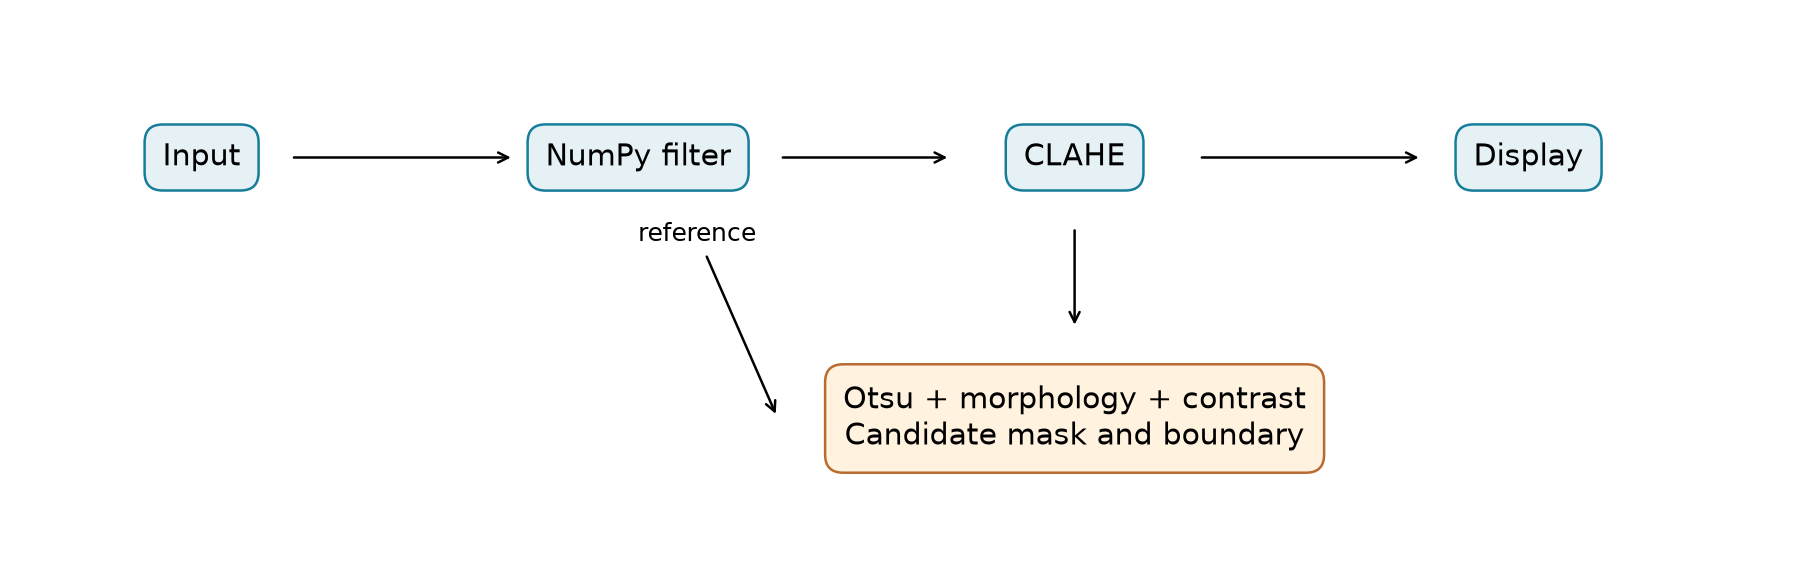
\includegraphics[width=\linewidth]{assets/pipeline.png}
Hình 3.1. Luồng dữ liệu của pipeline và nhánh ảnh tham chiếu.
\end{center}
Hình 3.1 cho thấy nhánh trước CLAHE được giữ riêng. Làm nét không thay đổi đầu vào phân đoạn. Giao diện hiển thị rõ kết quả nào là ảnh quan sát, bản đồ biên hoặc mask ứng viên; không biến số pixel biên thành diện tích vùng. Phân công trên là trách nhiệm từ phiên bản hiện tại, không xác nhận tác giả lịch sử.
\par
\clearpage
\section*{3.2. Cài đặt lọc không gian và bộ lọc SAR}
\textbf{Thuật toán 3.1. Các bộ lọc cục bộ (đầu vào I, cửa sổ lẻ k; đầu ra J)}
\begin{flushleft}
1. Kiểm tra ảnh hữu hạn, k lẻ; chuyển float trước phép trừ/nhân.\\
2. Đệm reflect-101; tính moment bằng tổng tích lũy cho Box, Lee, Kuan.\\
3. Box: J ← mean cửa sổ. Gaussian: hai lượt kernel 1D chuẩn hóa.\\
4. Median: J ← trung vị cửa sổ.\\
5. Bilateral: trọng số ← Gauss(khoảng cách) × Gauss(chênh mức xám).\\
6. Lee: tính K; Kuan: tính W từ Ci², Cu²; nội suy giữa mean và pixel.\\
7. Frost biến thể: trọng số exp(−a·CV·distance), chuẩn hóa tổng.\\
8. Round, clip 0..255 và chuyển uint8.\\
\end{flushleft}
Bảng 3.2 chỉ ra chi phí tăng theo cửa sổ và số pixel. Tổng tích lũy tránh lặp lại phép cộng cho mọi cửa sổ. Gaussian được tách theo hai chiều vì kernel là tích của hai kernel 1D. Median và Bilateral dùng sliding\_window\_view để biểu diễn cửa sổ; các phép nhân trung gian vẫn có thể cần O(Nk²) bộ nhớ, dù view tự nó không sao chép dữ liệu. Demo giới hạn k đến 9 để tránh chi phí không kiểm soát.
\par
\noindent\textit{Bảng 3.2. Chi phí nhóm lọc với N=H×W}
\begin{longtable}{p{4.87cm}|p{4.87cm}|p{4.87cm}}
Phương pháp & Thời gian & Bộ nhớ bổ sung\\\hline
Box/Lee/Kuan & O(N) & O(N)\\\hline
Gaussian tách & O(Nk) & O(N)\\\hline
Median & Phụ thuộc chọn trung vị từng cửa sổ & Có thể O(Nk²)\\\hline
Bilateral/Frost biến thể & O(Nk²) & O(Nk²) trung gian\\\hline
\end{longtable}
Code yêu cầu sigma và số look dương; cửa sổ phải lẻ. Trong đối chiếu, quy tắc biên của thư viện được đặt tương ứng. Khác biệt ở vùng mép do dùng reflect thay vì nearest không được bỏ qua bằng cách chỉ cắt vùng giữa và tuyên bố khớp toàn ảnh.
\par
\clearpage
\section*{3.3. Cài đặt biến đổi điểm, CLAHE và đồng hình}
\textbf{Thuật toán 3.2. Log, HE và CLAHE (đầu vào I và tham số; đầu ra J)}
\begin{flushleft}
1. Log: tạo LUT log1p cho 256 mức theo r\_max, tra LUT cho từng pixel.\\
2. HE: đếm histogram; cộng dồn CDF; xử lý riêng ảnh hằng.\\
3. CLAHE: đệm để kích thước chia hết cho lưới; tạo histogram mỗi tile.\\
4. Cắt histogram; chia lượng dư thành thương nguyên và phần dư.\\
5. Tạo LUT uint8 từ CDF với cùng quy tắc làm tròn.\\
6. Tính trọng số giữa tâm tile; nội suy bốn LUT cho từng pixel.\\
7. Trả ảnh kích thước gốc, không trả phần đệm.\\
\end{flushleft}
\textbf{Thuật toán 3.3. Lọc đồng hình (đầu vào I, γL, γH, c, D₀; đầu ra J)}
\begin{flushleft}
1. L ← log(1+I).\\
2. F ← FFT2(L); dịch gốc tần số về tâm.\\
3. Tạo H(u,v) từ khoảng cách tới tâm và các tham số.\\
4. Z ← phần thực của IFFT2(F×H) sau dịch ngược.\\
5. J ← exp(Z)−1; chuẩn hóa min/max về 0..255; xử lý ảnh hằng.\\
\end{flushleft}
Log và HE cần O(N+256) thời gian, bảng ánh xạ nhỏ. CLAHE cần O(N+256T) với T là số tile và thêm O(256T+N) bộ nhớ cho LUT, tọa độ và ảnh nội suy. Đồng hình dùng FFT có chi phí xấp xỉ O(N log N), bộ nhớ O(N) số phức. NumPy FFT được coi là phép toán số nền tảng; thuật toán lọc và ghép các bước do nhóm cài.
\par
Lưới 1×1 và ảnh không chia hết cho lưới là hai ca dễ gây chia cho 0 hoặc sai nội suy. Kiểm thử so trực tiếp với cv2.createCLAHE cả các ca đó. Không dùng kết quả CLAHE như bằng chứng rằng tín hiệu tối mới xuất hiện là đối tượng mới trong cảnh.
\par
\clearpage
\section*{3.4. Cài đặt làm nét và các toán tử biên}
\textbf{Thuật toán 3.4. Làm nét và gradient (đầu vào I; đầu ra ảnh làm nét/biên)}
\begin{flushleft}
1. Unsharp/high-boost: blur I; tính mask=I−blur; J=I+k·mask.\\
2. Laplacian sharpen: tính tổng bốn láng giềng−4I; J=I−α·L.\\
3. Roberts: tính hai chênh lệch chéo trên cửa sổ 2×2.\\
4. Prewitt/Sobel: tích chập tương quan với hai kernel đạo hàm.\\
5. G ← hypot(Gx,Gy), θ ← atan2(Gy,Gx).\\
6. Sobel enhancement: cộng 0,5G vào I để quan sát.\\
7. Chỉ round/clip ảnh hiển thị; giữ Gx,Gy float để xử lý tiếp.\\
\end{flushleft}
\textbf{Thuật toán 3.5. LoG và zero crossing}
\begin{flushleft}
1. Lấy bán kính ceil(3σ); tạo kernel LoG rồi trừ mean kernel.\\
2. Tương quan ảnh đã đệm reflect với kernel.\\
3. Đặt đáp ứng |L|<10⁻⁹ bằng 0 để bỏ đổi dấu do triệt tiêu số học.\\
4. Xét bốn cặp đối diện; giữ khi tích âm và chênh lệch vượt ngưỡng.\\
5. Trả bản đồ nhị phân 0/255.\\
\end{flushleft}
Đạo hàm kernel cố định có O(N) thời gian và O(N) bộ nhớ. LoG tổng quát có O(Nk²), với k phụ thuộc sigma. Khi so với filter2D, cần chỉ rõ anchor của kernel Roberts 2×2; nếu để anchor khác nhau, biên có thể lệch một pixel dù công thức kernel giống nhau. Đầu ra biên bị cắt về 255 chỉ là biểu diễn hiển thị, không thay cho độ lớn gradient dùng bên trong Canny.
\par
\clearpage
\section*{3.5. Cài đặt Canny và kiểm soát sai khác}
\textbf{Thuật toán 3.6. Canny tự cài (I, low, high, σ → biên nhị phân)}
\begin{flushleft}
1. Nếu thiếu ngưỡng: lấy ngưỡng từ median ảnh; kiểm tra 0≤low≤high.\\
2. Làm mịn Gaussian 5×5; tính Sobel float và góc hướng.\\
3. Lượng tử góc thành 0°,45°,90°,135°.\\
4. NMS: giữ pixel không nhỏ hơn hai láng giềng theo đúng hướng.\\
5. Mạnh: nms>0 và nms≥high; yếu: nms>0 và low≤nms<high.\\
6. Đưa pixel mạnh vào hàng đợi.\\
7. Duyệt BFS, nối pixel yếu 8-láng giềng chưa thăm.\\
8. Trả các pixel mạnh hoặc yếu đã nối thành ảnh 0/255.\\
\end{flushleft}
Hysteresis duyệt mỗi pixel tối đa một lần, nên thời gian O(N) sau bước gradient và bộ nhớ O(N) cho ảnh trạng thái/hàng đợi. NMS được vector hóa bằng các lát ảnh đệm. Bản cũ đưa độ lớn đã clip uint8 vào NMS; điều này làm các gradient lớn bão hòa bằng nhau và có thể giữ những vị trí không phải cực đại. Phiên bản hiện tại dùng hypot(Gx,Gy) float.
\par
Đối chứng OpenCV dùng ảnh đã được làm mịn giống nhau, bật L2gradient và cùng cặp ngưỡng. Tuy nhiên, quy tắc so sánh bằng nhau, lượng tử góc, cách xử lý mép của hai phiên bản không được giả định tương đương. Bảng xuất vì vậy giữ MSE, sai số lớn nhất, tỷ lệ pixel khớp và F1 biên chính xác vị trí để mô tả khác biệt; không tính các hàng này là PASS.
\par
Một phép kiểm tra tối thiểu là ảnh hằng ở ngưỡng 0 phải trả ảnh biên rỗng. Quy tắc nms>0 tránh biến mọi pixel bằng 0 thành cạnh mạnh. Kiểm tra ngưỡng đảo ngược phải báo lỗi thay vì âm thầm tạo đầu ra không có nghĩa.
\par
\clearpage
\section*{3.6. Phân đoạn, liên thông và lọc ứng viên}
\textbf{Thuật toán 3.7. Otsu, hình thái và phân đoạn vùng tối}
\begin{flushleft}
1. Otsu: histogram→xác suất→moment tích lũy→t cực đại phương sai giữa lớp.\\
2. Chọn ảnh tăng cường hoặc reference theo tỷ lệ tối và η; ghi đây là heuristic.\\
3. Nếu bật thích ứng và vùng tối >35\%, giảm t theo chênh mean hai lớp.\\
4. Mask ← I≤t; ảnh hằng cho mask rỗng.\\
5. Erosion/dilation: AND/OR các lát dịch theo kernel; ghép thành opening/closing.\\
6. Gán nhãn run-length union-find; lọc diện tích nhỏ.\\
7. Lấy vòng nền dilation(mask)−mask; đo CR trên reference.\\
8. Giữ mọi vùng đạt min\_contrast; không có vòng nền thì bỏ.\\
9. β(A) ← A−erosion(A); xuất vùng, diện tích, centroid, bounding box.\\
\end{flushleft}
\textbf{Thuật toán 3.8. Gán nhãn 8-liên thông bằng các đoạn chạy}
\begin{flushleft}
1. Mỗi hàng: tìm các đoạn foreground liên tiếp [left,right].\\
2. Tạo nhãn cho đoạn; nối với đoạn hàng trước có khoảng cách ≤1 pixel.\\
3. Union-find hợp nhất nhãn tương đương, nén đường đi.\\
4. Ánh xạ root thành nhãn liên tục; đếm diện tích bằng bincount.\\
5. Chỉ dựng mask metadata cho vùng qua min\_area; không thay ma trận nhãn.\\
\end{flushleft}
Ngưỡng Otsu được tính trong O(N+256), morphology O(N|B|). Gán nhãn theo đoạn có chi phí quét O(N) cộng hợp nhất các đoạn giao nhau; dựng mask cho K vùng được giữ có thể tốn O(KN) thời gian/bộ nhớ. Việc bỏ metadata cho vùng nhỏ giúp giảm chi phí thực tế, nhưng không được tuyên bố toàn pipeline O(N) khi K tăng. Đây là giới hạn cần nêu trong thiết kế.
\par
\clearpage
\section*{3.7. Kiểm chứng, xử lý lỗi và tích hợp Streamlit}
Bảng 3.3 phân biệt mức bằng chứng mà mỗi kiểu đối chứng cung cấp. TV2 tổ chức registry gồm tên phép toán, hàm tự cài, hàm tham chiếu, mô tả quy tắc biên và giới hạn sai số. Ba nhóm được tách rõ: API trực tiếp; phép ghép primitive thư viện; biến thể mô tả. Các ca gồm ảnh đen, trắng, hằng, ramp, checkerboard, đường chéo, nhiễu có seed, xung đơn và 10 ảnh mẫu. Khi có FAIL ở nhóm có giới hạn, lệnh tái tạo kết quả dừng với mã lỗi.
\par
\noindent\textit{Bảng 3.3. Quy tắc đối chứng}
\begin{longtable}{p{4.87cm}|p{4.87cm}|p{4.87cm}}
Nhóm & Ví dụ & Diễn giải\\\hline
Trực tiếp & HE, CLAHE, Sobel, Otsu, morphology & Cùng tham số, dtype và border\\\hline
Phép ghép & Lee/Kuan/Frost, homomorphic, sharpen & Kiểm tra công thức bằng primitive; không có API toàn thuật toán tương đương\\\hline
Biến thể & Bilateral, Canny & Giữ sai khác và phân tích; không tính là PASS\\\hline
\end{longtable}
Kiểm thử hồi quy còn kiểm tra phân hoạch liên thông so OpenCV, tham số không hợp lệ, endpoint của Otsu, ảnh hằng và bất biến mask khi đổi làm nét. Kiểm tra AST phát hiện import thư viện đối chứng trong các module lõi TV3/TV4/metrics TV5. Đây là hàng rào kiến trúc, không thay thế đọc mã hoặc chứng minh toán học.
\par
Streamlit có các tab kết quả ảnh, chỉ số, bảng đối chứng và phân công. Người dùng chọn ảnh mẫu hoặc tải tệp, thay bộ lọc và tham số, tải PNG/JSON. AppTest kiểm tra luồng mặc định, đổi Canny và quay lại morphology, chọn ảnh 00013; đó là kiểm tra hành vi giao diện, không phải chứng nhận tương thích mọi trình duyệt. Những ảnh lỗi giải mã hoặc tham số không hợp lệ được thông báo thay vì trả kết quả giả.
\par
\noindent\textit{Bảng 3.4. Lệnh và sản phẩm}
\begin{longtable}{p{7.3cm}|p{7.3cm}}
Lệnh & Sản phẩm\\\hline
uv sync --locked --all-extras & Môi trường Python theo uv.lock\\\hline
uv run python reproduce.py & CSV, JSON, ảnh chẩn đoán trong results/\\\hline
uv run --extra dev python -m pytest tests -q & Kiểm thử hồi quy và ranh giới thư viện\\\hline
uv run streamlit run streamlit\_app.py & Demo tương tác tại localhost:8501\\\hline
\end{longtable}
Bảng 3.4 phục vụ kiểm tra giao diện và tái lập từ cùng môi trường; kết quả chạy được lưu riêng với dữ liệu đầu vào.
\par
\clearpage
\section*{4.1. Môi trường và quy trình tái lập}
\noindent\textit{Bảng 4.1. Môi trường của lần đo}
\begin{longtable}{p{7.3cm}|p{7.3cm}}
Thuộc tính & Giá trị\\\hline
Python & 3.13.5\\\hline
Hệ điều hành & Windows-11-10.0.26100-SP0\\\hline
CPU / logical CPUs & Intel64 Family 6 Model 154 Stepping 3, GenuineIntel / 16\\\hline
RAM vật lý & 15.7 GiB\\\hline
NumPy / OpenCV & 2.5.4 / 5.0.0\\\hline
Seed / process dataset & 2026 / 4\\\hline
Ngày chạy & 2026-11-11T21:36:42+0700\\\hline
Hash mã nguồn (rút gọn) & 28ecff90ac5cd28b2c2547ee\\\hline
scipy & 1.18.1\\\hline
scikit-image & 0.26.0\\\hline
matplotlib & 3.11.2\\\hline
pandas & 3.1.1\\\hline
streamlit & 1.67.0\\\hline
\end{longtable}
Bảng 4.1 ghi môi trường đã khóa; lệnh tái lập nằm ở mục 3.7 và phụ lục A. Các số liệu trong chương này được đọc từ file CSV/JSON sau khi chạy reproduce.py, không gõ lại bằng tay. Manifest lưu commit nền, trạng thái working tree, SHA-256 của mã nguồn, seed và cấu hình pipeline. Khi working tree có sửa đổi, chỉ ghi commit là chưa đủ tái lập; hash nguồn giúp nhận diện đúng trạng thái đã đo.
\par
Một lệnh chạy toàn bộ gồm ví dụ số, đối chiếu thư viện, thực nghiệm bộ mẫu và đánh giá hai lớp dataset. Tùy chọn --samples-only phục vụ phát triển nhưng phải được ghi rõ là phạm vi hạn chế. Thời gian từng ảnh được đo bằng đồng hồ đơn điệu; benchmark dataset dùng nhiều process nên số mili giây có ảnh hưởng tranh chấp tài nguyên, không được coi là độ trễ một yêu cầu độc lập trên máy nhàn rỗi.
\par
\clearpage
\section*{4.2. Dữ liệu, nhãn và thiết kế thí nghiệm}
\noindent\textit{Bảng 4.2. Tập ảnh trong dự án}
\begin{longtable}{p{4.87cm}|p{4.87cm}|p{4.87cm}}
Tập & Số ảnh & Vai trò\\\hline
Class\_0 & 3.695 & Đánh giá mức ảnh theo nhãn thư mục\\\hline
Class\_1 & 1.843 & Đánh giá mức ảnh theo nhãn thư mục\\\hline
Mẫu demo & 10 & 5 dầu + 5 biển; chạy khảo sát và đối chứng\\\hline
Ảnh tổng hợp & 8 & Điều kiện biên và kiểm chứng số học\\\hline
\end{longtable}
Bảng 4.2 phân biệt dữ liệu đánh giá, demo và ca tổng hợp. Nguồn [13] được xác định từ kaggle/metadata/dataset\_metadata.xml: CSIRO, David Blondeau-Patissier, ngày 15/12/2022, DOI 10.25919/4v55-dn16. Metadata mô tả chip Sentinel-1 xám JPEG 400×400, nhãn 0 là biển sạch/look-alike và 1 có dầu. Tệp license.html đi kèm ghi CC BY-SA 4.0. Tên bộ dữ liệu có nhắc ML/DL nhưng việc dùng các ảnh cho thí nghiệm xử lý ảnh không yêu cầu huấn luyện mô hình.
\par
Metadata công bố 5.630 ảnh (3.725 lớp 0, 1.905 lớp 1); repo có 5.538 ảnh khác nhau, thiếu 30 ảnh lớp 0 và 62 ảnh lớp 1. Không có checksum gốc để giải thích chênh lệch. Ảnh 400×400 lưu RGB, pipeline đọc xám. Ngoài hai lớp chính, kaggle/data/sample có 10 bản sao trùng byte: 5.548 đường dẫn nhưng 5.538 ảnh khác nhau, không đếm lặp khi đánh giá. Cả 10 ảnh demo cũng khớp byte với dataset; đây là tập con khảo sát, không phải tập đánh giá độc lập. Chưa có mask pixel hoặc định danh cảnh để kiểm tra chồng lấn giữa các chip.
\par
Thí nghiệm A hỏi các bộ lọc thay đổi biến thiên và thành phần biên ra sao. Thí nghiệm B khảo sát CLAHE theo clip 1–5 và grid 4/8/16. Thí nghiệm C thêm nhiễu Gauss σ=10,20,30 cùng ảnh sạch để quan sát độ nhạy của bộ dò biên. Thí nghiệm D phân tích 00013 và toàn bộ năm ảnh biển mẫu. Thí nghiệm E đo sự có mặt của vùng ứng viên trên toàn bộ hai lớp.
\par
Không có bước huấn luyện và không tối ưu tham số trên một tập test rồi gọi đó là đánh giá độc lập. Các thí nghiệm nhỏ dùng cùng 10 ảnh nên chỉ hỗ trợ nhận xét trên bộ mẫu, không đại diện mọi điều kiện SAR. Nhiễu Gauss được dùng như điều kiện bất lợi có thể tái lập, không thay thế mô hình speckle nhân của dữ liệu gốc.
\par
\clearpage
\section*{4.3. Kết quả đối chiếu: lọc và tăng cường}
\noindent\textit{Bảng 4.3. Sai số lớn nhất và MSE trung bình trên 18 ca}
\begin{longtable}{p{3.65cm}|p{3.65cm}|p{3.65cm}|p{3.65cm}}
Phép toán & Nhóm đối chứng & Max |Δ| & MSE TB\\\hline
box & Trực tiếp & 0 & 0\\\hline
gaussian & Trực tiếp & 0 & 0\\\hline
median & Trực tiếp & 0 & 0\\\hline
bilateral & Biến thể & 20 & 2.01\\\hline
lee & Ghép hàm & 0 & 0\\\hline
frost & Ghép hàm & 0 & 0\\\hline
kuan & Ghép hàm & 0 & 0\\\hline
log & Ghép hàm & 0 & 0\\\hline
HE & Trực tiếp & 0 & 0\\\hline
CLAHE & Trực tiếp & 1 & 0.00013\\\hline
homomorphic & Ghép hàm & 0 & 0\\\hline
\end{longtable}
Bảng 4.3 phân biệt so trực tiếp API và đối chiếu bằng primitive. Các phép Box, Gaussian, Median đặt border tương ứng trước khi so. Gaussian cho phép sai khác một mức xám do thứ tự tính và làm tròn. HE cần riêng trường hợp hằng; CLAHE cần thống nhất giới hạn histogram, phần dư và nội suy. Sự giống nhau của các phép biến đổi này không chứng minh chúng cải thiện phân đoạn dầu.
\par
Lee, Kuan và Frost biến thể được tính lại bằng moment/shift của SciPy và công thức đã trình bày. Đây là đối chứng cấu thành: nếu cả hai cùng dùng một giả định mô hình không phù hợp dữ liệu thì vẫn có thể khớp số học. Homomorphic dùng scipy.fft làm đối chứng chuỗi biến đổi. Bilateral dùng footprint khác nên được giữ ở trạng thái DESCRIPTIVE, không nâng ngưỡng tùy ý để đổi thành PASS.
\par
Các giá trị trong bảng là tổng hợp của sai số từng ca; bảng per\_case.csv giữ lại cả ảnh tổng hợp lẫn ảnh thật. Có thể truy ngược một sai khác tới ảnh, phương pháp và thông số. Báo cáo không chỉ chọn ảnh khớp đẹp để trình bày.
\par
\clearpage
\section*{4.4. Kết quả đối chiếu: biên, hình thái và metrics}
\noindent\textit{Bảng 4.4. Đối chiếu nhóm biên và hình thái}
\begin{longtable}{p{3.65cm}|p{3.65cm}|p{3.65cm}|p{3.65cm}}
Phép toán & Nhóm đối chứng & Max |Δ| & MSE TB\\\hline
unsharp & Ghép hàm & 0 & 0\\\hline
high\_boost & Ghép hàm & 0 & 0\\\hline
laplacian\_sharpen & Ghép hàm & 0 & 0\\\hline
sobel\_enhance & Ghép hàm & 0 & 0\\\hline
roberts & Ghép hàm & 0 & 0\\\hline
prewitt & Ghép hàm & 0 & 0\\\hline
sobel & Trực tiếp & 0 & 0\\\hline
LoG & Ghép hàm & 0 & 0\\\hline
canny & Biến thể & 255 & 32.8\\\hline
otsu & Trực tiếp & 0 & 0\\\hline
erosion & Trực tiếp & 0 & 0\\\hline
dilation & Trực tiếp & 0 & 0\\\hline
opening & Ghép hàm & 0 & 0\\\hline
closing & Ghép hàm & 0 & 0\\\hline
boundary & Ghép hàm & 0 & 0\\\hline
components & Trực tiếp & 0 & 0\\\hline
\end{longtable}
\noindent\textit{Bảng 4.5. Đối chiếu sáu chỉ số định lượng}
\begin{longtable}{p{3.65cm}|p{3.65cm}|p{3.65cm}|p{3.65cm}}
Phép toán & Nhóm đối chứng & Max |Δ| & MSE TB\\\hline
ENL & Ghép hàm & 4.02e-11 & 1.17e-22\\\hline
SSI & Ghép hàm & 0 & 0\\\hline
RMS & Trực tiếp & 2.96e-13 & 9.85e-27\\\hline
entropy & Ghép hàm & 7.08e-07 & 5.44e-14\\\hline
AMBE & Ghép hàm & 2.84e-14 & 5.61e-29\\\hline
EPI & Ghép hàm & 0 & 0\\\hline
\end{longtable}
Bảng 4.4 và Bảng 4.5 liệt kê sai số nhóm biên, hình thái và chỉ số. Sobel/Prewitt so cả Gx và Gy ở float thay vì chỉ ảnh độ lớn bão hòa. Roberts đặt anchor rõ cho kernel 2×2. LoG đặt đáp ứng gần zero bằng 0 ở cả hai phép tính để tránh khác dấu do triệt tiêu số học. Otsu chọn ngưỡng đầu tiên đạt cực đại và kiểm tra I≤t; hai điều này tránh sai khác endpoint bị che bởi ảnh xám hiển thị.
\par
Nhãn thành phần liên thông có thể khác thứ tự đánh số mà vẫn mô tả cùng phân hoạch. Bộ kiểm tra hồi quy xác nhận ánh xạ một-một giữa các vùng; bảng đo dùng diện tích vùng tại từng pixel như một đại lượng bất biến theo ID. Với erosion/dilation, giá trị ngoài ảnh được đặt rõ ràng để không so hai quy ước khác nhau.
\par
Canny vẫn là đối chiếu biến thể, không có lời kết luận “khớp tuyệt đối”. Sáu metrics cũng có đối chứng riêng, nhưng chúng chỉ đo các đặc tính đã định nghĩa. MSE=0 của entropy hoặc EPI không có nghĩa đường biên đúng với thực tế. Tổng số PASS/DESCRIPTIVE trong toàn bộ registry được báo trên bảng tổng hợp kèm theo.
\par
\clearpage
\section*{4.5. So sánh bộ lọc: giảm biến thiên và mất chi tiết}
\noindent\textit{Bảng 4.6. SSI và EPI, trung bình ± độ lệch chuẩn trên 10 ảnh}
\begin{longtable}{p{4.87cm}|p{4.87cm}|p{4.87cm}}
Bộ lọc & SSI (TB ± SD) & EPI (TB ± SD)\\\hline
none & 1.0000 ± 0.0000 & 1.0000 ± 0.0000\\\hline
box & 0.9313 ± 0.1065 & 0.4784 ± 0.1797\\\hline
gaussian & 0.9596 ± 0.0654 & 0.5840 ± 0.1181\\\hline
median & 0.9423 ± 0.0983 & 0.6783 ± 0.1588\\\hline
bilateral & 0.9456 ± 0.0812 & 0.5679 ± 0.1282\\\hline
lee & 0.9314 ± 0.1065 & 0.4792 ± 0.1793\\\hline
frost & 0.9342 ± 0.1033 & 0.4884 ± 0.1723\\\hline
kuan & 0.9313 ± 0.1065 & 0.4790 ± 0.1794\\\hline
\end{longtable}
Bảng 4.6 in đậm SSI trung bình nhỏ nhất và EPI trung bình gần 1 nhất trong các bộ lọc (loại hàng ảnh gốc khỏi xếp hạng). Đó là hai tiêu chí riêng, không phải kết luận một bộ lọc tối ưu đồng thời cho khử nhiễu và phân đoạn.
\par
SSI nhỏ hơn 1 cho thấy hệ số biến thiên toàn ảnh giảm so ảnh đầu vào. EPI gần 1 có nghĩa tổng đáp ứng Laplacian được giữ theo định nghĩa của chỉ số; nó không tách được biên thật khỏi nhiễu. Vì vậy không thể chọn bộ lọc tốt nhất chỉ từ một cột. Khi SSI giảm đồng thời EPI giảm nhiều, cần xem vùng chuyển tiếp trước khi kết luận lợi ích.
\par
Kết quả bộ mẫu cho thấy Lee, Kuan và Box có các giá trị gần nhau trong cấu hình khảo sát. Điều này phù hợp với cơ chế khi trọng số thích nghi nhỏ: kết quả tiến gần trung bình cục bộ. Không có căn cứ nói Lee luôn bảo toàn biên tốt nhất. Median và Gaussian cho đánh đổi khác, tùy phân bố cường độ và kết cấu của từng ảnh.
\par
ENL có thể tăng rất mạnh khi ROI góc trên trở nên gần hằng. Đây là dấu hiệu cần xem lại ROI, không phải bằng chứng số look vật lý tăng tương ứng. Bảng nguồn giữ ENL và thời gian để người đọc kiểm tra; thời gian đang đo toàn pipeline với cùng cấu hình phân đoạn, không phải chỉ thời gian riêng kernel lọc. Độ lệch chuẩn lớn cần được giữ lại, không chỉ báo trung bình.
\par
\clearpage
\section*{4.6. Khảo sát CLAHE và độ nhạy tham số}
\begin{center}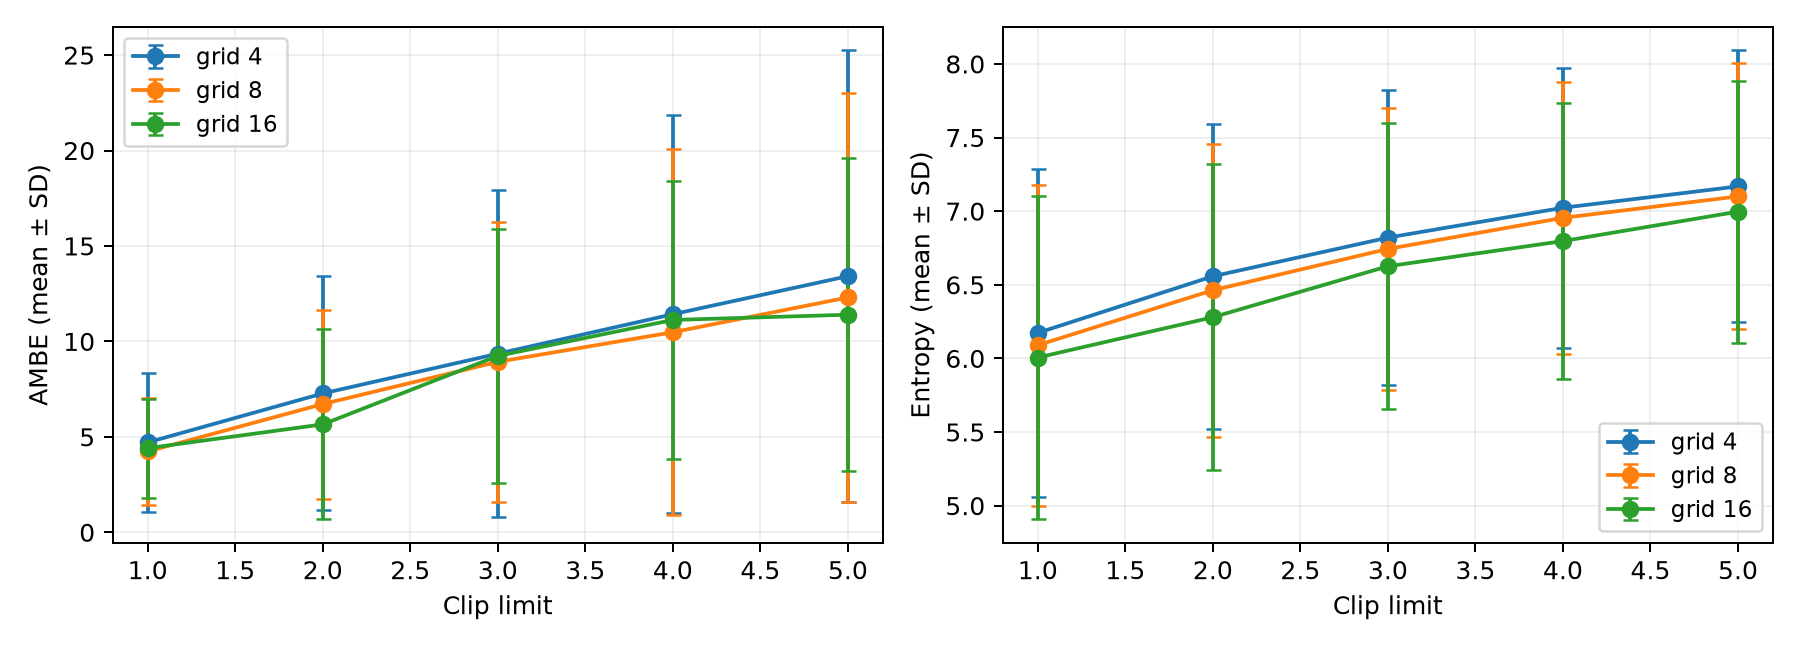
\includegraphics[width=\linewidth]{assets/clahe_survey.png}
Hình 4.1. AMBE và entropy trung bình theo clip và grid trên bộ mẫu.
\end{center}
Bảng 4.7 là lát cắt clip=2 của khảo sát ở Hình 4.1. Hình 4.1 giúp trả lời tham số CLAHE thay đổi độ sáng và phân bố mức xám như thế nào. Mỗi điểm được tổng hợp từ cùng 10 ảnh. Clip và grid là hai yếu tố khác nhau: clip điều chỉnh cắt histogram, grid thay đổi kích thước vùng thống kê. Tăng entropy sau biến đổi không tự chứng minh vùng dầu được tách tốt hơn.
\par
\noindent\textit{Bảng 4.7. Một số cấu hình tại clip=2}
\begin{longtable}{p{4.87cm}|p{4.87cm}|p{4.87cm}}
Grid & AMBE (TB ± SD) & Entropy (TB ± SD)\\\hline
4 & 7.273 ± 6.129 & 6.558 ± 1.034\\\hline
8 & 6.717 ± 4.953 & 6.463 ± 0.996\\\hline
16 & 5.654 ± 4.970 & 6.280 ± 1.039\\\hline
\end{longtable}
Mask cuối có thể ít thay đổi giữa hai cấu hình khi quy tắc chọn ảnh phân đoạn chuyển sang reference trước CLAHE. Vì thế cần báo cả ảnh tăng cường, tỷ lệ vùng ứng viên và ảnh thực sự được dùng để phân đoạn, không suy luận từ histogram hiển thị duy nhất. Không chọn thông số dựa vào vẻ đẹp của một ảnh rồi coi đó là tối ưu trên toàn dataset.
\par
\clearpage
\section*{4.7. Điều kiện bất lợi: nhiễu và mật độ biên}
\begin{center}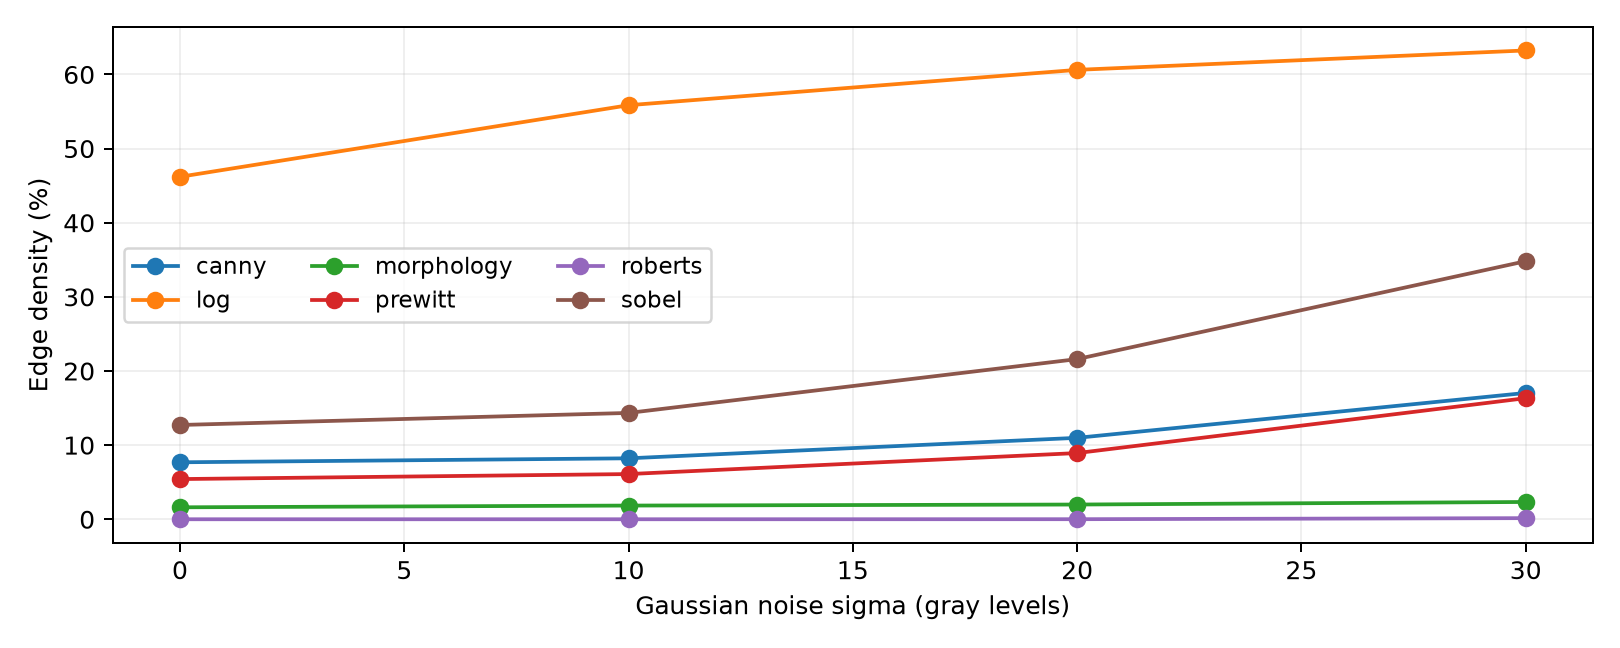
\includegraphics[width=\linewidth]{assets/edge_noise.png}
Hình 4.2. Mật độ biên theo mức nhiễu Gauss, trung bình trên bộ mẫu.
\end{center}
Hình 4.2 cho biết mỗi phương pháp phản ứng thế nào khi đầu vào thay đổi. Mật độ biên là tỷ lệ pixel khác 0 trong bản đồ biên; không phải precision/recall vì chưa có nhãn biên chuẩn. Một phương pháp trả rất ít biên có thể đã bỏ sót đối tượng, còn nhiều biên có thể do nền hoặc nhiễu. Cần đối chiếu đồng thời ảnh và chỉ số.
\par
Nhiễu được sinh bằng bộ sinh số giả ngẫu nhiên với seed 2026. Mỗi ảnh ở mỗi mức có một realization; phương pháp biên được chạy trên cùng ảnh nhiễu ở mức đó để so sánh công bằng. Độ lệch chuẩn hiện tại là giữa các ảnh, không phải khoảng tin cậy trên nhiều lần sinh nhiễu. Nếu cần kết luận ổn định theo nhiễu, cần lặp nhiều seed và tách hai nguồn biến thiên.
\par
Việc tự thêm Gauss là điều kiện thử kiểm soát được, không nói ảnh SAR gốc chỉ có nhiễu Gauss. Kết quả được dùng để giải thích hạn chế của đạo hàm và ngưỡng hóa, đúng mục tiêu phân tích điều kiện bất lợi của học phần. Thời gian của Canny có thể tăng khi số điểm mạnh/yếu và độ liên thông tăng.
\par
\clearpage
\section*{4.8. Ca 00013 và các ảnh biển bị nhận nhầm}
\begin{center}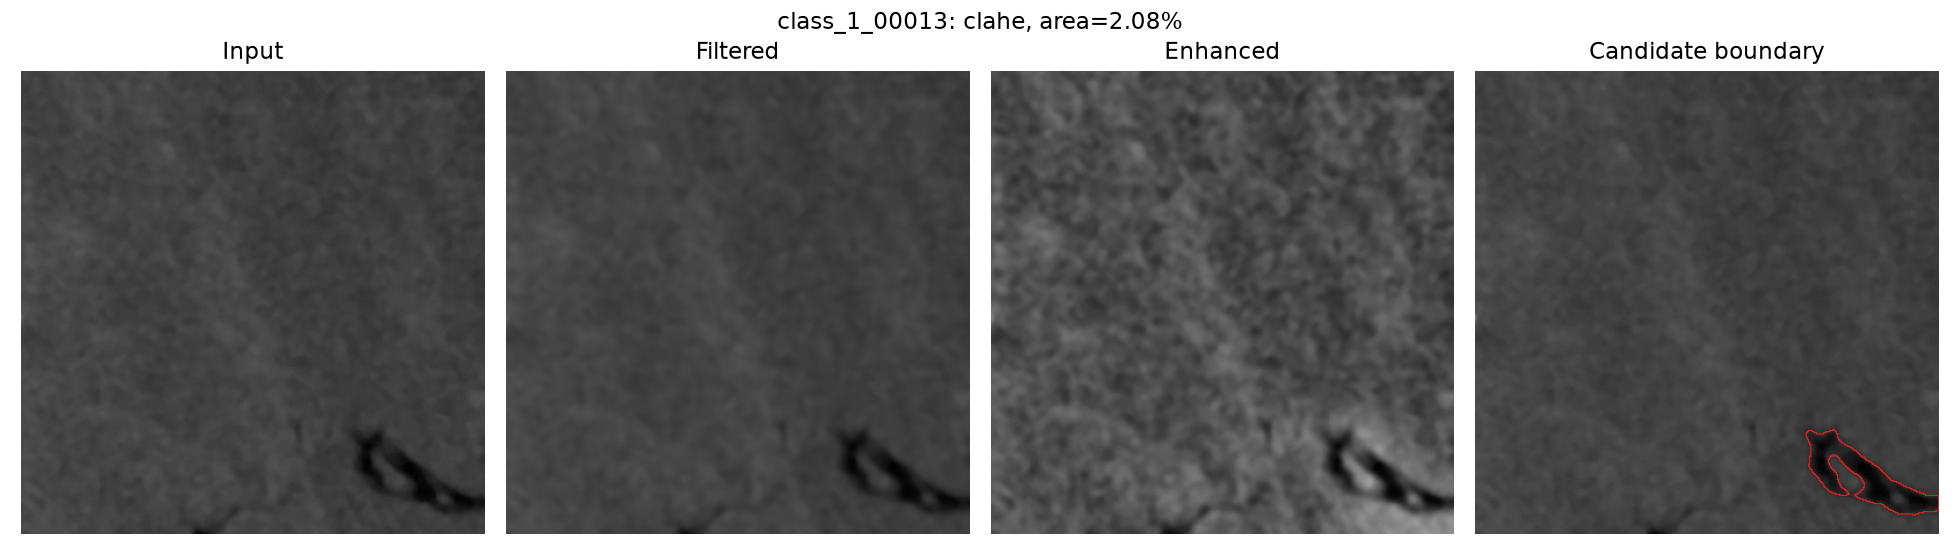
\includegraphics[width=\linewidth]{assets/class_1_00013_clahe.png}
Hình 4.3. Ảnh 00013: đầu vào, ảnh lọc, CLAHE và biên ứng viên.
\end{center}
\begin{center}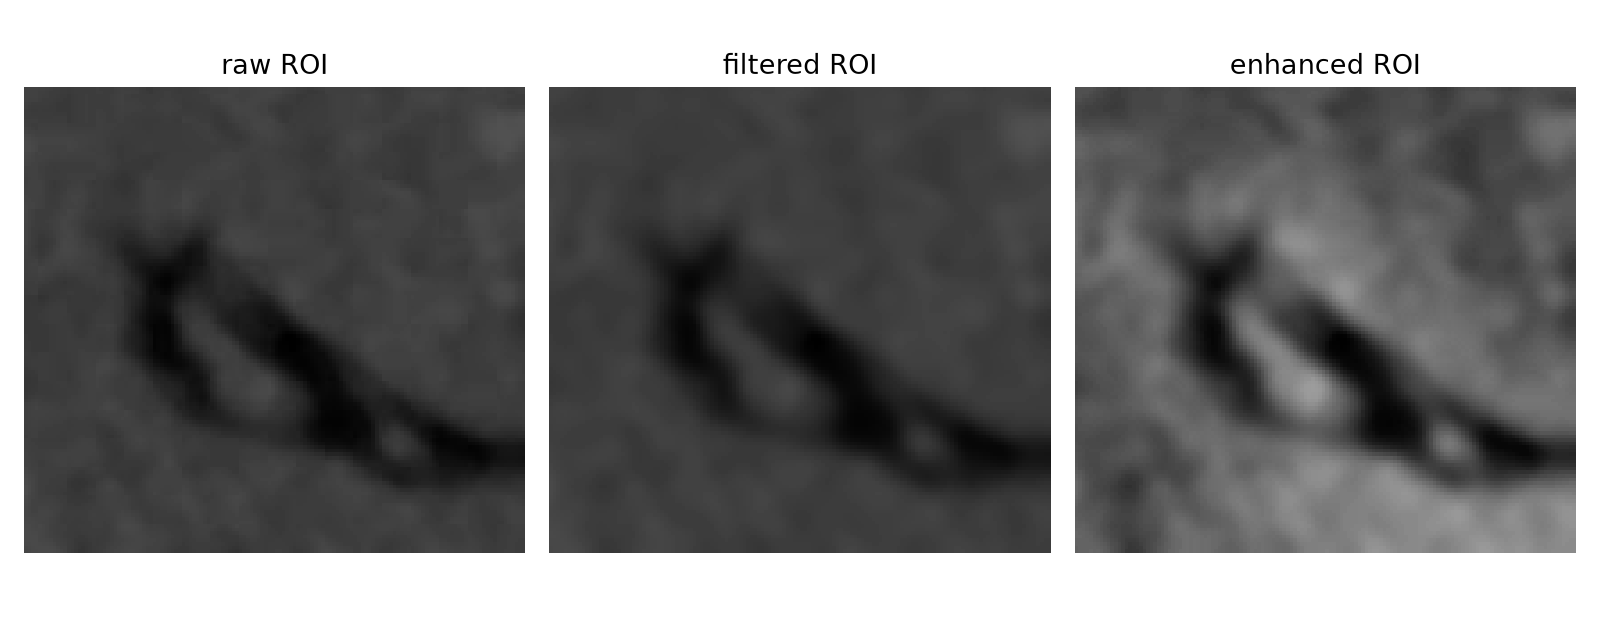
\includegraphics[width=\linewidth]{assets/roi_00013.png}
Hình 4.4. Cùng ROI vệt chính trên ảnh gốc, ảnh lọc và ảnh tăng cường.
\end{center}
Hình 4.4 phóng to vệt chính; Bảng 4.8 cho thấy các ảnh biển vẫn có báo nhầm. Với cấu hình mặc định hiện tại, ảnh 00013 giữ 1 vùng ứng viên, chiếm 2.08\% ảnh, CR trung bình 0.520. Hình 4.3–4.4 cho thấy vệt chính nổi bật hơn, nhưng chưa có mask chuẩn để lượng hóa độ khớp. Trong năm ảnh biển mẫu, 3/5 ảnh vẫn có ứng viên; do đó không thể kết luận lọc đã loại hết báo động giả.
\par
CLAHE làm rõ cả dao động nền vốn khó thấy bằng mắt; Otsu lại tối ưu phân tách mức xám chứ không tối ưu nhãn dầu. Nếu mask trước đó nhận nền thành một vùng lớn có lỗ, phép lấy biên sẽ vẽ cả mép các lỗ. Đây là lý do nhiều vòng nhỏ trên hình không nhất thiết biểu thị nhiều đối tượng riêng. Lỗi gán nhãn chủ yếu phát sinh ở phân đoạn; bước lấy biên chỉ phản ánh mask đó.
\par
\noindent\textit{Bảng 4.8. Ảnh biển mẫu, cấu hình CLAHE mặc định}
\begin{longtable}{p{4.87cm}|p{4.87cm}|p{4.87cm}}
Ảnh biển & Số vùng & Diện tích (\%)\\\hline
sea\_surface\_01 & 2 & 19.31\\\hline
sea\_surface\_02 & 3 & 31.72\\\hline
sea\_surface\_03 & 0 & 0.00\\\hline
sea\_surface\_04 & 0 & 0.00\\\hline
sea\_surface\_05 & 4 & 16.38\\\hline
\end{longtable}
\begin{center}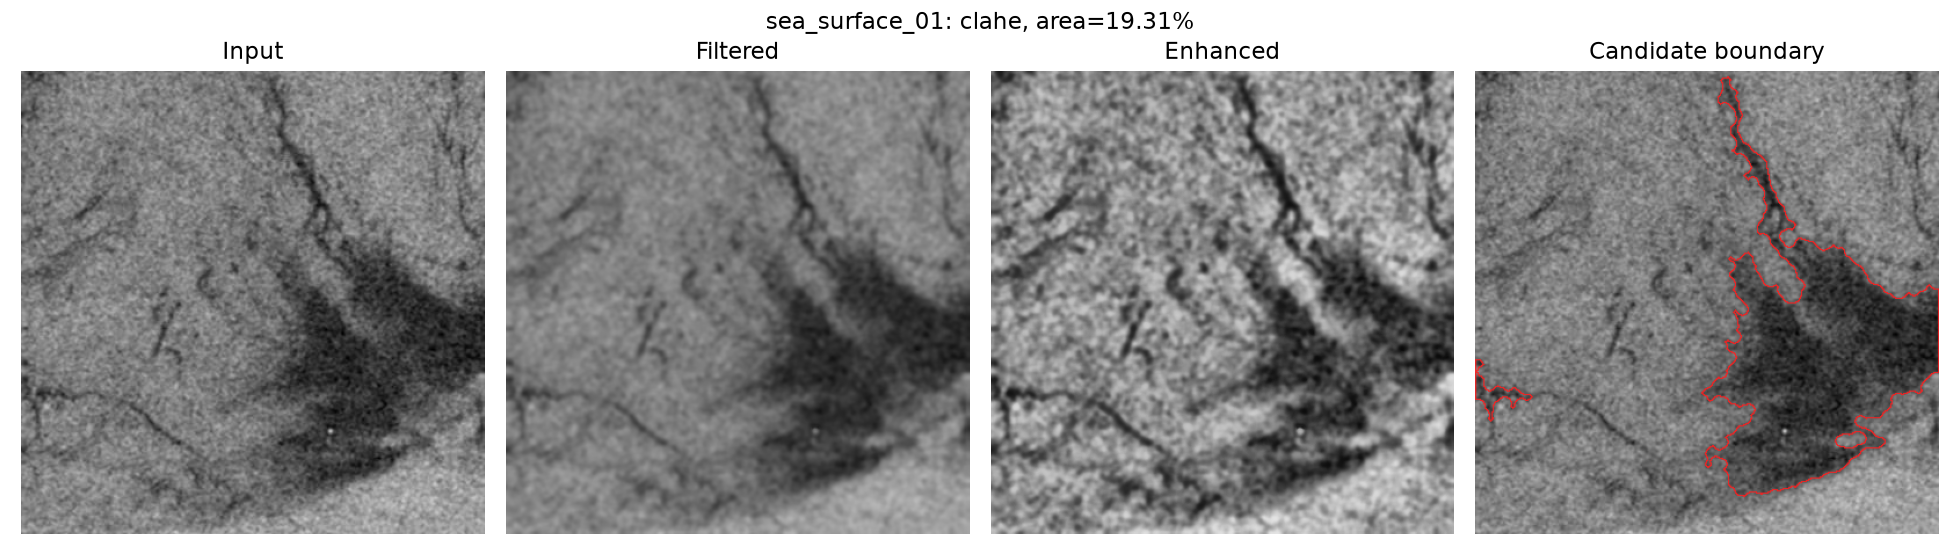
\includegraphics[width=\linewidth]{assets/sea_surface_01_clahe.png}
Hình 4.5. Ca báo nhầm sea\_surface\_01: vùng nền tối được giữ thành ứng viên.
\end{center}
Hình 4.5 là ví dụ thất bại ở ảnh được đặt trong nhóm biển. Hai vùng qua được các kiểm tra diện tích và tương phản vì các tiêu chí đó mô tả hình học/mức xám, không kiểm chứng bản chất dầu. Closing có thể nối nền tối thành vùng lớn. Vì vậy lọc diện tích đơn thuần không đủ sửa loại báo nhầm này; cần đánh giá quy tắc nền cục bộ và mask gán tay như đề xuất ở chương 5.
\par
\clearpage
\section*{4.9. Đánh giá cấp ảnh trên cả hai lớp}
\noindent\textit{Bảng 4.9. Ma trận nhầm lẫn theo nhãn thư mục}
\begin{longtable}{p{4.87cm}|p{4.87cm}|p{4.87cm}}
Nhãn thật theo thư mục & Không có ứng viên & Có ứng viên\\\hline
Class\_0 & 810 & 2885\\\hline
Class\_1 & 204 & 1639\\\hline
\end{longtable}
\noindent\textit{Bảng 4.10. Chỉ số cấp ảnh và phạm vi diễn giải}
\begin{longtable}{p{7.3cm}|p{7.3cm}}
Chỉ số & Giá trị\\\hline
Precision & 36.23\%\\\hline
Recall & 88.93\%\\\hline
F1 & 51.48\%\\\hline
Specificity & 21.92\%\\\hline
Accuracy cấp ảnh & 44.22\%\\\hline
\end{longtable}
Bảng 4.9 và Bảng 4.10 phải được đọc cùng phạm vi nhãn cấp ảnh. Quy tắc dự đoán dương tính là có ít nhất một vùng tối được giữ. Kết quả cho thấy nhiều ảnh Class\_0 cũng có vùng thỏa diện tích và tương phản, nên độ đặc hiệu còn thấp. Đây là hạn chế của quy tắc dựa vào cường độ và hình thái, không thể sửa bằng cách đổi nhãn heuristic thành “sạch chuẩn”. Tỷ lệ phát hiện cao ở Class\_1 phải được đọc cùng số báo nhầm.
\par
Precision=TP/(TP+FP), Recall=TP/(TP+FN), F1=2TP/(2TP+FP+FN), Specificity=TN/(TN+FP), Accuracy=(TP+TN)/N. Các chỉ số này dựa trên giả định ý nghĩa nhãn thư mục và ở cấp ảnh. Không có giá trị IoU/Dice hoặc sai số diện tích thực vì thiếu mask, độ phân giải mặt đất và xác minh vật lý.
\par
Không loại các ca xấu khỏi mẫu đánh giá và không dùng tập này để khẳng định hiệu năng triển khai ngoài thực tế. Tất cả 5.538 đường dẫn được lưu ở bảng per\_image; số ảnh mỗi lớp được kiểm tra trước tổng hợp. Bước tiếp theo có căn cứ là xây dựng nhãn vùng trên một tập đại diện và đối chiếu các quy tắc nền cục bộ, không phải tăng độ mạnh CLAHE để làm hình bắt mắt hơn.
\par
\clearpage
\section*{5.1. Đối chiếu mục tiêu và kết quả đạt được}
\noindent\textit{Bảng 5.1. Đối chiếu mục tiêu chương 1}
\begin{longtable}{p{4.87cm}|p{4.87cm}|p{4.87cm}}
Mục tiêu & Kết quả & Giới hạn\\\hline
M1: lõi NumPy & Đã triển khai và có kiểm tra ranh giới import & FFT dùng primitive NumPy; I/O/resize ở lớp tích hợp\\\hline
M2: kiểm chứng & 5 ví dụ; 33 thuật toán/chỉ số ×18 ca & 558 PASS, 36 DESCRIPTIVE; không phải mọi thuật toán có API độc lập\\\hline
M3: demo & Streamlit, AppTest và xuất PNG/JSON & Chưa là kiểm thử mọi trình duyệt/tệp ảnh\\\hline
M4: tái lập & Một lệnh, kết quả từng ảnh, manifest/hash & CSIRO có metadata/giấy phép; chưa rõ 92 ảnh chênh lệch\\\hline
M5: hồ sơ nhóm & Phân công, báo cáo, slide, mẫu đánh giá & Tên đã cung cấp; MSSV/chữ ký chờ điền; video đang hoãn\\\hline
\end{longtable}
Bảng 5.1 đối chiếu từng mục tiêu M1–M5 với bằng chứng và giới hạn. Kết quả đạt được quan trọng nhất là pipeline có thể giải thích và kiểm chứng từng phần. Báo cáo đã sửa cách hiểu C\_R, tách làm nét khỏi phân đoạn và loại lời kết luận tuyệt đối từ một heuristic. Các sửa lỗi số học như endpoint Otsu, ảnh hằng, gradient float và gần-zero LoG được gắn với kiểm thử tái hiện, thay vì chỉ mô tả bằng lời.
\par
Mặt khác, khả năng nhận diện dầu từ vùng tối chưa đạt mức đủ tin cậy cho vận hành. Số báo nhầm toàn tập là bằng chứng trực tiếp cho giới hạn này. Học phần có thể đánh giá việc cài đặt, phân tích và cải tiến theo phạm vi đã đăng ký; báo cáo không tự thay giảng viên kết luận điểm hoặc mức đạt của cả nhóm.
\par
\clearpage
\section*{5.2. Hạn chế và hướng phát triển khả thi}
Bảng 5.2 đề xuất các bước kiểm tra cụ thể cho ba hướng cải tiến. Hạn chế dữ liệu gồm JPEG không có thông tin hiệu chuẩn bức xạ đi kèm mỗi ảnh, thiếu mask pixel, ít hơn bộ CSIRO công bố 92 ảnh và chưa xác định các chip có cùng cảnh chụp. Hạn chế thuật toán gồm ngưỡng toàn cục, ROI ENL cố định, vòng nền có thể chứa vùng ứng viên khác và tham số diện tích phụ thuộc resize. Hạn chế thực nghiệm gồm bộ mẫu nhỏ cho khảo sát tham số, một realization mỗi mức nhiễu và benchmark chạy song song có ảnh hưởng thời gian.
\par
\noindent\textit{Bảng 5.2. Ba hướng tiếp tục trong xử lý ảnh truyền thống}
\begin{longtable}{p{7.3cm}|p{7.3cm}}
Hướng & Cách kiểm tra đề xuất\\\hline
Ước lượng nền cục bộ & So sánh vòng nền loại trừ vùng ứng viên với nền toàn cục; giữ tập đánh giá riêng\\\hline
Phân đoạn đa tỉ lệ & Khảo sát cửa sổ và phép hình thái theo độ phân giải; đánh giá bỏ sót/nhận nhầm\\\hline
Gán mask tập đại diện & Nhóm khoanh vùng độc lập, thống nhất bất đồng; tính IoU/Dice và sai số biên\\\hline
\end{longtable}
Những hướng này không đòi hỏi ML/DL. Nếu thử thêm một quy tắc lọc mới, cần nêu giả thuyết, tham số và tiêu chí trước khi xem kết quả trên tập đánh giá. Một cải thiện về precision có thể làm giảm recall; cần báo cả hai thay vì chỉ lựa chỉ số thuận lợi. Bổ sung mask chỉ phục vụ đánh giá nếu không dùng để huấn luyện mô hình.
\par
Trước khi nộp, nhóm cần điền MSSV và xác nhận đóng góp, kiểm tra nguồn tham khảo, bổ sung hồ sơ dữ liệu và diễn tập 12 phút trình bày, 3 phút demo, 5 phút vấn đáp. Nhật ký hồi cứu phải ghi đúng ngày bổ sung và minh chứng, không sửa lịch sử commit. Video chưa thực hiện theo yêu cầu hiện tại; điểm và nhận xét trong bảng đánh giá chéo được để trống để từng thành viên tự điền.
\par
\clearpage
\section*{Tài liệu tham khảo}
[1] Bộ môn Xử lý ảnh, UTC, “ds btl xla VÀ HƯỚNG DẪN,” tài liệu hướng dẫn BTL trong dự án, không ghi năm.
\par
[2] C. Brekke and A. H. S. Solberg, “Oil spill detection by satellite remote sensing,” Remote Sensing of Environment, vol. 95, pp. 1–13, 2005, doi:10.1016/j.rse.2004.11.015.
\par
[3] K. Topouzelis, “Oil spill detection by SAR images: Dark formation detection, feature extraction and classification algorithms,” Sensors, vol. 8, pp. 6642–6659, 2008, doi:10.3390/s8106642.
\par
[4] J.-S. Lee, “Digital image enhancement and noise filtering by use of local statistics,” IEEE TPAMI, vol. PAMI-2, pp. 165–168, 1980, doi:10.1109/TPAMI.1980.4766994.
\par
[5] A. M. Reza, “Realization of the contrast limited adaptive histogram equalization (CLAHE) for real-time image enhancement,” Journal of VLSI Signal Processing Systems, vol. 38, pp. 35–44, 2004, doi:10.1023/B:VLSI.0000028532.53893.82.
\par
[6] J. Canny, “A computational approach to edge detection,” IEEE TPAMI, vol. PAMI-8, pp. 679–698, 1986, doi:10.1109/TPAMI.1986.4767851.
\par
\clearpage
\section*{Tài liệu tham khảo (tiếp)}
[7] N. Otsu, “A threshold selection method from gray-level histograms,” IEEE TSMC, vol. 9, pp. 62–66, 1979, doi:10.1109/TSMC.1979.4310076.
\par
[8] D. T. Kuan et al., “Adaptive noise smoothing filter for images with signal-dependent noise,” IEEE TPAMI, vol. PAMI-7, pp. 165–177, 1985, doi:10.1109/TPAMI.1985.4767641.
\par
[9] V. S. Frost et al., “A model for radar images and its application to adaptive digital filtering of multiplicative noise,” IEEE TPAMI, vol. PAMI-4, pp. 157–166, 1982, doi:10.1109/TPAMI.1982.4767223.
\par
[10] R. C. Gonzalez and R. E. Woods, Digital Image Processing, 4th ed. Pearson, 2018.
\par
[11] OpenCV, “Image processing reference,” tài liệu thư viện, https://docs.opencv.org/4.x/d7/dbd/group\_\_imgproc.html. Đối chứng thực tế dùng phiên bản ghi trong manifest.
\par
[12] SciPy, “Multidimensional image processing (scipy.ndimage),” tài liệu thư viện, https://docs.scipy.org/doc/scipy/reference/ndimage.html. Đối chứng thực tế dùng phiên bản ghi trong manifest.
\par
[13] D. Blondeau-Patissier, CSIRO Sentinel-1 SAR image dataset of oil- and non-oil features for machine learning (Deep Learning), CSIRO, Dec. 15, 2022, doi:10.25919/4v55-dn16. Nguồn và CC BY-SA 4.0 theo metadata/giấy phép kèm repo; số ảnh bản cục bộ khác số công bố.
\par
Danh mục dùng định dạng đánh số IEEE theo thứ tự xuất hiện. Metadata bài báo kế thừa hồ sơ tham khảo của dự án; nhóm cần mở bản gốc và kiểm tra lại trích dẫn trước nộp. Trong đợt này không truy cập nguồn ngoài dự án để xác minh giấy phép hay nội dung từng bài.
\par
\clearpage
\section*{Phụ lục A. Tái lập và truy nguyên kết quả}
Repo: https://github.com/hotung9108/utc-sar-oil-detection. Mã mới phải được commit theo ngày thực khi nhóm quyết định bàn giao; báo cáo ghi thêm hash nguồn vì lần chạy có working tree thay đổi.
\par
\noindent\textit{Các vị trí cần tra cứu}
\begin{longtable}{p{7.3cm}|p{7.3cm}}
Nội dung & Đường dẫn từ gốc dự án\\\hline
Môi trường & pyproject.toml; uv.lock; .python-version\\\hline
Ví dụ tính tay & src/tv2/verification.py\\\hline
Đối chiếu tất cả kết quả & src/tv2/library\_comparison.py\\\hline
Thực nghiệm và lớp dữ liệu & src/tv5/experiments.py\\\hline
Bằng chứng đông cứng & docs/report/evidence/\\\hline
Slide và lời trình bày & docs/slides/\\\hline
Nhật ký và đánh giá chéo & docs/management/PHAN\_CONG\_VA\_MINH\_CHUNG\_BTL.xlsx\\\hline
\end{longtable}
Tại thư mục gốc: uv sync --locked --all-extras; uv run python reproduce.py; uv run --extra docs python scripts/build\_report.py; uv run --extra docs python scripts/build\_defense\_slides.py. Mở demo bằng uv run streamlit run streamlit\_app.py. Dùng Python 3.13; script PDF dùng font Times New Roman của Windows để hỗ trợ tiếng Việt.
\par
File checksums.json đi kèm evidence cho phép đối chiếu tệp bảng đã dùng. Không chỉnh tay giá trị CSV để thay đổi kết luận. Nếu sửa mã thuật toán hoặc tham số thí nghiệm, chạy lại một lệnh tái lập rồi dựng lại báo cáo và slide.
\par
\clearpage
\section*{Phụ lục B. Mã kiểm chứng ví dụ số}
Mã đầy đủ gọi trực tiếp thuật toán đang dùng: https://github.com/hotung9108/utc-sar-oil-detection/blob/main/src/tv2/verification.py. File tương ứng trong repo là src/tv2/verification.py; chạy uv run python -m src.verification. Bảng kết quả có trong docs/report/evidence/verification\_hand\_examples.json.
\par
Ví dụ 4×4 HE: ma trận gồm bốn hàng [0,0,0,0], [1,1,1,1], [2,2,2,2], [3,3,3,3]. Histogram [4,4,4,4], CDF [4,8,12,16]. LUT = round(255·(CDF−4)/(16−4)) = [0,85,170,255]. Cài đặt được gọi là global\_histogram\_equalization; sai số lớn nhất so kết quả tính tay bằng 0.
\par
Ví dụ 5×5 Lee: toàn ma trận bằng 100, riêng ô giữa bằng 200. Cửa sổ 3×3 quanh tâm có tám giá trị 100 và một giá trị 200. μ=1000/9; E[I²]=120000/9; σ²=E[I²]−μ²=80000/81. Với L=4, μ²/L lớn hơn σ² nên K=0; đầu ra tâm round(1000/9)=111. Kết quả đã kiểm chứng bằng NumPy qua custom\_lee\_filter.
\par
Ba fixture còn lại kiểm tra đạo hàm Sobel, diện tích erosion/dilation và ngưỡng Otsu. Kết quả kỳ vọng là hằng số tính trước, không lấy chính hàm đang kiểm tra làm đáp án. Bất kỳ ví dụ sai nào khiến lệnh kiểm chứng dừng với lỗi; không ghi PASS khi chỉ dựng được bảng.
\par
\clearpage
\section*{Phụ lục C. Nhật ký nhóm và sử dụng AI}
Nhật ký 8 tuần trong tài liệu cũ là nội dung cần xác minh, không phải bằng chứng công việc đã thực hiện. Khung hồi cứu 16/09–10/11/2026 có 40 dòng TV1–TV5; nội dung đề xuất, ghi nhận cũ và minh chứng Git được tách riêng. Quy định chung ghi 3 tuần thực hiện trong khi phần mã nguồn yêu cầu 8 tuần commit; nhóm cần hỏi giảng viên cách áp dụng.
\par
Excel đánh giá chéo có 20 cặp khác người. Họ tên do nhóm cung cấp và tài khoản GitHub được đối chiếu với collaborators; MSSV, phần trăm đóng góp, điểm và chữ ký chờ nhóm điền. Tài liệu học, trình bày và câu hỏi từng người nằm trong docs/thanh\_vien/. Khung hồi cứu bổ sung từ 10/08 đến 11/11/2026 ghi đúng ngày lập, không tạo lịch sử Git giả.
\par
Công cụ hỗ trợ trong đợt cập nhật: Codex qua ứng dụng. Phạm vi gồm đọc yêu cầu, rà mã, sửa lỗi, tổ chức module, tạo demo, đối chiếu thư viện, chạy thực nghiệm, tổng hợp báo cáo và tạo slide bằng mã. Các công cụ AI được tài liệu cũ nhắc tới cần nhóm xác nhận lại mức sử dụng thực tế; không mặc nhiên coi mọi khai báo cũ đã được kiểm chứng.
\par
Cách kiểm tra gồm kiểm thử hồi quy, số liệu đối chiếu từng ca, manifest, hash nguồn, kiểm tra PDF/slide và đối chiếu cấu trúc. Những kiểm tra tự động không thay thế việc sinh viên đọc công thức, hiểu mã, xác nhận nguồn và diễn tập bảo vệ. Nhóm cần ghi rõ những phần đã kiểm tra thực tế, người kiểm tra và ngày xác nhận.
\par
Kịch bản bảo vệ: 12 phút trình bày theo slide, 3 phút thao tác demo và 5 phút vấn đáp. Video 5–7 phút chưa tạo theo yêu cầu hiện tại. Các phần cá nhân và video là đầu việc còn lại trước khi nộp bộ hồ sơ đầy đủ.
\par
\end{document}